\documentclass[11pt,a4paper]{article}
% =============================================================================
% Preamble — typography, math, tables, bibliography
% =============================================================================

\usepackage[a4paper, margin=2.4cm, footskip=1cm]{geometry}
\usepackage[utf8]{inputenc}
\usepackage[T1]{fontenc}
\usepackage{lmodern}
\usepackage{microtype}
\usepackage{setspace}
\onehalfspacing

\usepackage{amsmath, amssymb, mathtools, amsthm}
\usepackage{bm}
\usepackage{booktabs}
\usepackage{multirow}
\usepackage{array}
\usepackage{siunitx}
\sisetup{group-separator={\,}, group-minimum-digits=4, output-decimal-marker={.}}
\usepackage{graphicx}
\graphicspath{{figures/}{../artifacts/figures/}}
\usepackage{caption}
\captionsetup{font=small, labelfont=bf, labelsep=period}
\usepackage{subcaption}
\usepackage{xcolor}
\usepackage[hidelinks]{hyperref}
\hypersetup{
  pdftitle  = {Selling Property Rental Ownership: A Multi-Model Tranche-Pricing Study of Paris Residential Rent},
  pdfauthor = {Dan Allouche},
  pdfsubject = {Quantitative finance — credit risk, structured products, real estate},
  pdfkeywords = {tranche pricing, CDO, copula, Vasicek, Merton, Monte Carlo, Paris real estate},
}
\usepackage[capitalise, noabbrev]{cleveref}
\usepackage[round, sort&compress]{natbib}
\bibliographystyle{plainnat}
% Provide a \autocite alias for compatibility with the biblatex-style calls
% in the section files.
\newcommand{\autocite}[1]{\citep{#1}}
\usepackage{eurosym}
\providecommand{\EUR}{\euro}
\usepackage{tikz}
\usetikzlibrary{positioning, arrows.meta, calc}

% --- Theorem-like environments ---------------------------------------------- %
\newtheorem{definition}{Definition}[section]
\newtheorem{assumption}[definition]{Assumption}
\newtheorem{proposition}[definition]{Proposition}

% --- Math macros ------------------------------------------------------------ %
\newcommand{\R}{\mathbb{R}}
\newcommand{\N}{\mathbb{N}}
\newcommand{\E}{\mathbb{E}}
\newcommand{\Prob}{\mathbb{P}}
\newcommand{\Var}{\operatorname{Var}}
\newcommand{\Cov}{\operatorname{Cov}}
\newcommand{\dW}{\mathrm{d}W}
\newcommand{\dt}{\mathrm{d}t}
\newcommand{\given}{\mid}
\DeclareMathOperator{\VaR}{VaR}
\DeclareMathOperator{\ES}{ES}
\DeclareMathOperator*{\argmin}{arg\,min}

% --- Author block ----------------------------------------------------------- %
\title{\bfseries\Large Selling Property Rental Ownership\\
  \large\itshape A Multi-Model Tranche-Pricing Study of Paris Residential Rent}
\author{Dan Allouche}
\date{May 2026}

\newcommand{\dataParisStart}{1992-03-31}
\newcommand{\dataParisEnd}{2025-12-31}
\newcommand{\dataParisN}{136}
\newcommand{\dataOatN}{796}
\newcommand{\paramGbmMu}{3.35\%}
\newcommand{\paramGbmSigma}{4.08\%}
\newcommand{\paramVasicekA}{0.0163}
\newcommand{\paramVasicekB}{4.40\%}
\newcommand{\paramVasicekSigma}{0.78\%}
\newcommand{\parTotal}{31.5~M\EUR}
\newcommand{\nObligors}{70}
\newcommand{\nPaths}{50000}
\newcommand{\horizonYears}{10}
\newcommand{\pdTerminal}{26.3\%}
\newcommand{\rhoBaseline}{0.15}
\newcommand{\fairToParModela}{1.107}
\newcommand{\sharpeModela}{-2.16}
\newcommand{\meanReturnModela}{0.95\%}
\newcommand{\probNegModela}{22.9\%}
\newcommand{\fairToParModelb}{0.908}
\newcommand{\sharpeModelb}{-2.43}
\newcommand{\meanReturnModelb}{-1.13\%}
\newcommand{\probNegModelb}{70.1\%}
\newcommand{\fairToParEquity}{1.030}
\newcommand{\sharpeEquity}{-0.66}
\newcommand{\meanReturnEquity}{-1.15\%}
\newcommand{\probNegEquity}{52.2\%}
\newcommand{\fairToParMezzanine}{0.786}
\newcommand{\sharpeMezzanine}{-1.78}
\newcommand{\meanReturnMezzanine}{-2.82\%}
\newcommand{\probNegMezzanine}{98.7\%}
\newcommand{\fairToParSenior}{0.939}
\newcommand{\sharpeSenior}{-21.26}
\newcommand{\meanReturnSenior}{-0.63\%}
\newcommand{\probNegSenior}{100.0\%}
\newcommand{\seniorFairGauss}{0.939}
\newcommand{\seniorFairStudent}{0.934}
\newcommand{\seniorFairCox}{0.896}
\newcommand{\insuranceAnnualPremium}{746~k\EUR}
\newcommand{\insuranceExpectedLoss}{6326~k\EUR}
\newcommand{\insuranceCoverage}{90\%}


\begin{document}
\maketitle

\begin{abstract}\noindent
We study a hybrid real-estate investment structure in which the rental cash
flows of a Paris residential building are partitioned into a senior /
mezzanine / equity tranche stack akin to a synthetic CDO, and compare its
risk-return profile to two classical benchmarks: outright single-apartment
ownership (Model A) and a fully pooled SAS share (Model B). All market
parameters are calibrated on French sources: \dataParisN{} quarterly observations of the
Notaires-INSEE price index (\dataParisStart{}--\dataParisEnd{}), the INSEE
\textit{Indice de Référence des Loyers}, and the French ten-year sovereign
yield (FRED \texttt{IRLTLT01FRM156N}). Default times are simulated under
three benchmark credit models — the Gaussian one-factor copula
\autocite{Li2000, Vasicek2002}, the Student-t copula
\autocite{EmbrechtsMcNeilStraumann2002} and a Cox doubly-stochastic
intensity \autocite{DuffieSingleton2003} — coupled with a Vasicek short rate
\autocite{Vasicek1977} and a geometric Brownian motion (with a Merton
jump-diffusion extension \autocite{Merton1976}) for the property value. The
tranche cash flows follow the Andersen-Sidenius-Basu (2003) waterfall and
are priced by Monte Carlo with antithetic variance reduction and a Sobol
QMC variant. On the Paris-intermediate scenario the senior fair value drops from
\seniorFairGauss{} of par under the Gaussian copula to
\seniorFairStudent{} under the Student-t copula, and the senior fair
coupon widens by roughly twelve basis points --- a numerical
illustration of the tail-dependence critique levelled at Li-style
models post-2008 \autocite{DonnellyEmbrechts2010, MacKenzieSpears2014}.
\end{abstract}


\begin{figure}[h!]
  \centering
  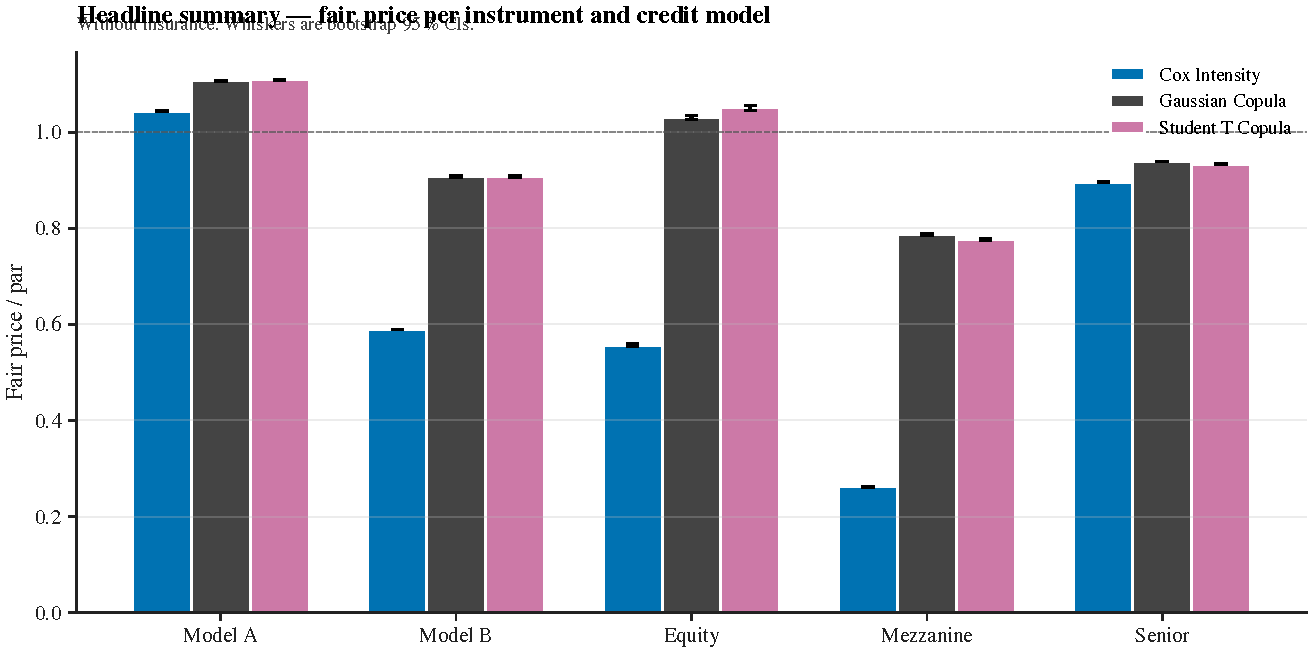
\includegraphics[width=0.95\linewidth]{fig_headline_summary.pdf}
\end{figure}

\clearpage
\tableofcontents
\clearpage

\section{Introduction}\label{sec:intro}

French residential real estate is an idiosyncratic asset class for
retail investors. The price process mean-reverts slowly; the rental
cash flow is heterogeneous and exposed to tenant-specific default risk;
and the legal framework around eviction, the \textit{Indice de Référence
des Loyers} and the Visale guarantee shapes realised loss in ways that
do not map cleanly onto traded credit instruments.

This paper asks whether, given the same underlying building, a tranched
cash-flow structure can deliver a different risk-return profile from
outright ownership or a classical SAS pool. We formalise three
investment vehicles --- Model A: single-apartment ownership; Model B: a
pro-rata SAS share; Model C: a CDO-style senior / mezzanine / equity
tranche stack --- and compute their fair price and risk metrics on the
same set of Monte Carlo paths.

The simulation pipeline is calibrated on \dataParisN{} quarters of
Notaires-INSEE Paris price data and \dataOatN{} months of OAT 10Y data;
every numerical estimate quoted in the paper is traceable to a row of
\texttt{artifacts/results.csv} produced by the same code. The credit
layer juxtaposes the Gaussian one-factor copula
\autocite{Li2000, Vasicek2002}, the Student-t copula
\autocite{EmbrechtsMcNeilStraumann2002}, and a Cox doubly stochastic
intensity \autocite{DuffieSingleton2003}, so the tail dependence that
the Gaussian benchmark silently sets to zero becomes visible at the
senior attach point. The rental-default insurance is priced both by the
actuarial standard-deviation principle and as a put on rent shortfall,
and the gap between the two is reported.

\subsection{Literature context}

The CDO tranching mechanic borrows from two modelling traditions. The
structural side originates with \autocite{BlackScholes1973} and
\autocite{Merton1976}: a firm defaults when its asset value crosses a
threshold, with the asset following a geometric Brownian motion. The
reduced-form side, started by \autocite{DuffieSingleton2003} and
expanded by \autocite{Schonbucher2003}, treats default as the first
jump of a Cox process driven by an exogenous hazard. The Cox
doubly-stochastic credit model in \cref{ssec:cox} is the canonical
example of the reduced-form mechanic with a CIR-like macro factor.

Copula-based pricing of multi-name credit baskets took off with
\autocite{Li2000}, which mapped default times into a joint Gaussian
distribution; \autocite{Vasicek2002} provided the large-portfolio
closed form that became the industry workhorse for CDO tranche pricing.
\autocite{EmbrechtsMcNeilStraumann2002} pointed out that the Gaussian
copula misses tail dependence, and \autocite{DonnellyEmbrechts2010}
quantified the implication for senior-tranche pricing in the subprime
crisis. \autocite{MacKenzieSpears2014} traces the Li (2000) formula's
twin role as industry standard and post-crisis scapegoat. The
Student-t copula benchmark in \cref{ssec:t-copula} is the alternative
that this strand of literature recommends.

The waterfall mechanic follows \autocite{AndersenSideniusBasu2003}: a
notional-depleting senior / mezzanine / equity stack with separate
interest and principal cascades. The contribution of the paper is not
in the modelling primitives, which are standard; it is in the
consistent calibration of those primitives on the public French
residential-rent dataset, juxtaposed with two retail benchmarks
(single-apartment ownership and a SAS pooled share) on a shared Monte
Carlo seed. The variance-reduction tooling follows
\autocite{Glasserman2003} for antithetic sampling and
\autocite{Owen1997} for scrambled Sobol QMC; risk measurement uses the
coherent expected-shortfall framework of \autocite{AcerbiTasche2002}.

\section{The three investment vehicles}\label{sec:models}

Throughout the paper we model a residential building made of $n$
independent rental units, observed over a horizon $T$ years. The building's
total par value at inception is $P_0$. Each apartment $i \in \{1, \ldots,
n\}$ has a stochastic default time $\tau_i$ with cumulative probability
$\Prob(\tau_i \le T) = p$ matched to a calibrated marginal hazard. The
fraction $\ell_i \in [0, 1]$ of par lost when apartment $i$ defaults is
drawn from a Beta distribution. The aggregate cumulative loss path is
\begin{equation}
L(t) = \frac{1}{n}\sum_{i = 1}^{n} \ell_i \,\mathbb{1}\{\tau_i \le t\},
\qquad t \in [0, T].
\label{eq:agg-loss}
\end{equation}
The building generates a net rental flow $R_t = (g - m)\, S_t\,(1 - L(t))$
in monetary units, where $S_t$ is the market value, $g$ is the gross
rental yield and $m$ the maintenance cost share, both expressed per year.

\paragraph{Model A — Classical full ownership.}
A single investor owns one apartment of the building (par $P_0 / n$). Cash
flows in period $[t, t + \Delta t]$ are $R_t\, \Delta t / n$ while
$\tau_1 > t$ and $0$ thereafter. At $T$ the apartment is sold at the
prevailing market value $S_T / n$ regardless of any past default.

\paragraph{Model B — SAS shareholders.}
$n$ investors each buy one share of a SAS that holds the whole building.
Each share receives the pro-rata net rent
$R_t\, \Delta t / n$ each period and $S_T (1 - L(T)) / n$ at terminal.

\paragraph{Model C — CDO-like tranches.}
The same aggregate cash flow $R_t$ is partitioned across a stack of
tranches $\tau = (\tau_\text{equity}, \tau_\text{mezz}, \tau_\text{senior})$
with attach / detach points $(0, 0.25)$, $(0.25, 0.60)$ and $(0.60, 1.00)$.
Tranche $\tau$ absorbs the cumulative loss via the stop-loss payoff
\begin{equation}
L_\tau(t) = \min\bigl(\max(L(t) - a_\tau, 0), d_\tau - a_\tau\bigr),
\label{eq:stop-loss}
\end{equation}
and the periodic net rent is allocated waterfall-style: senior coupon
first, then mezzanine, then equity collects the residual. At terminal the
sale proceeds $S_T (1 - L(T))$ are paid back to surviving notionals in the
same order.

\begin{assumption}\label{ass:par}
Total portfolio par is $P_0 = \nObligors \times 45\,\text{m}^2 \times
10\,000\,\EUR / \text{m}^2 = \parTotal$ for the Paris-intermediate scenario
that drives every numerical result reported below.
\end{assumption}

\section{Market dynamics}\label{sec:dynamics}

\subsection{Property price}

The building's market value $S_t$ follows geometric Brownian motion under
the physical measure:
\begin{equation}
\mathrm{d}S_t = \mu\, S_t\, \dt + \sigma\, S_t\, \dW_t.
\label{eq:gbm}
\end{equation}
By Itô's lemma applied to $f(S) = \log S$,
\begin{equation*}
\mathrm{d}\log S_t = \bigl(\mu - \tfrac{1}{2}\sigma^2\bigr)\dt + \sigma\, \dW_t,
\end{equation*}
so $\log S_{t + \Delta t} - \log S_t \sim \mathcal{N}\bigl((\mu - \sigma^2/2)\Delta t,\ \sigma^2 \Delta t\bigr)$
exactly. The maximum-likelihood estimator on $n$ equally-spaced
log-returns $r_i$ is therefore in closed form:
\begin{equation*}
\hat\sigma^2 = \frac{\mathrm{Var}(r)}{\Delta t},
\qquad
\hat\mu = \frac{\bar r}{\Delta t} + \tfrac{1}{2}\hat\sigma^2,
\end{equation*}
with asymptotic standard errors $\mathrm{SE}(\hat\sigma) =
\hat\sigma / \sqrt{2(n - 1)}$ and a delta-method extension for $\hat\mu$.
\Cref{eq:gbm} is discretised by exact log-Euler:
$S_{t + \Delta t} = S_t \exp\bigl( (\mu - \sigma^2 / 2)\Delta t + \sigma
\sqrt{\Delta t}\, Z \bigr)$, $Z \sim \mathcal{N}(0, 1)$. Parameters are
estimated by closed-form MLE on the quarterly log-return series of the
Notaires-INSEE Paris flats index (\dataParisN{} quarters, \dataParisStart{}
through \dataParisEnd{}). The fitted point estimates --- summarised in
\cref{tab:calibration} --- are $\hat\mu = \paramGbmMu{}$ and $\hat\sigma =
\paramGbmSigma{}$, with the visual diagnostics of \cref{fig:calib} indicating
mild departure from normality in the lower tail.

As a robustness extension we also estimate the Merton (1976)
jump-diffusion in which $S_t$ is augmented by a compound-Poisson jump
component $\sum_{k=1}^{N_t} (J_k - 1)$ with $N_t \sim \text{Poisson}(\lambda)$
and $\log J_k \sim \mathcal{N}(\mu_J, \sigma_J^2)$. Numerical MLE on the
truncated Poisson-mixture density does not deliver a likelihood improvement
on the Paris sample (see \cref{tab:calibration}): with $\hat\lambda$
collapsing close to $0$ and $\hat\sigma_J$ close to $0$, the jump
component is not separately identified. The empirical signature of
volatility clustering in the squared log-returns (\cref{fig:calib}, panel
d) is present at the first lags but the sample is too short for the
jump-diffusion parameters to be separately recovered. We retain GBM as
the baseline and note this finding explicitly.

\subsection{Short rate}

Discounting and option-theoretic insurance pricing both depend on a
stochastic short rate. We adopt the Vasicek (1977) model
\begin{equation}
\mathrm{d}r_t = a (b - r_t)\, \dt + \sigma_r\, \dW_t,
\label{eq:vasicek}
\end{equation}
whose transition law is Gaussian with closed form
\begin{equation*}
r_{t + \Delta t} \mid r_t \sim \mathcal{N}\!\left(
b + (r_t - b) e^{-a \Delta t},\
\tfrac{\sigma_r^2}{2 a}\bigl(1 - e^{-2 a \Delta t}\bigr)
\right).
\end{equation*}
Equivalently, $r_{t + \Delta t} = \alpha + \beta r_t + \varepsilon_t$
with $\beta = e^{-a \Delta t}$, $\alpha = b(1 - \beta)$ and
$\varepsilon_t \sim \mathcal{N}\bigl(0, \tfrac{\sigma_r^2}{2 a}(1 - \beta^2)\bigr)$ — an
AR(1) representation whose OLS estimator is the exact MLE. We invert
the mapping to recover $(a, b, \sigma_r)$ and report analytical standard
errors via the delta method. The closed-form zero-coupon bond price
\begin{equation*}
P(t, T \mid r_t) = \exp\bigl(A(t, T) - B(t, T) r_t\bigr),
\quad B(t, T) = \frac{1 - e^{-a(T - t)}}{a},
\end{equation*}
\begin{equation*}
A(t, T) = \Bigl(b - \tfrac{\sigma_r^2}{2 a^2}\Bigr)\bigl(B(t, T) - (T - t)\bigr) - \tfrac{\sigma_r^2 B(t, T)^2}{4 a},
\end{equation*}
is used in the option-theoretic insurance pricing of
\cref{sec:insurance}. The MLE is run on monthly France 10-year sovereign
yields (FRED \texttt{IRLTLT01FRM156N}, \dataOatN{} observations). The fitted estimates
are $\hat a = \paramVasicekA{}$, $\hat b = \paramVasicekB{}$ and
$\hat\sigma_r = \paramVasicekSigma{}$. The implied mean-reversion half-life
is decades; for a ten-year horizon this is effectively a near-random-walk,
which reflects the secular decline of European rates from the 1980s to
2020. Negative rates are permitted, consistent with the Eurozone reality of
2015--2022.

\Cref{fig:price-index} plots the Notaires-INSEE Paris price index used as
the empirical anchor for $\mu, \sigma$; the embedded inset shows the
quarterly log-returns that drive the calibration.

\begin{figure}[ht]
  \centering
  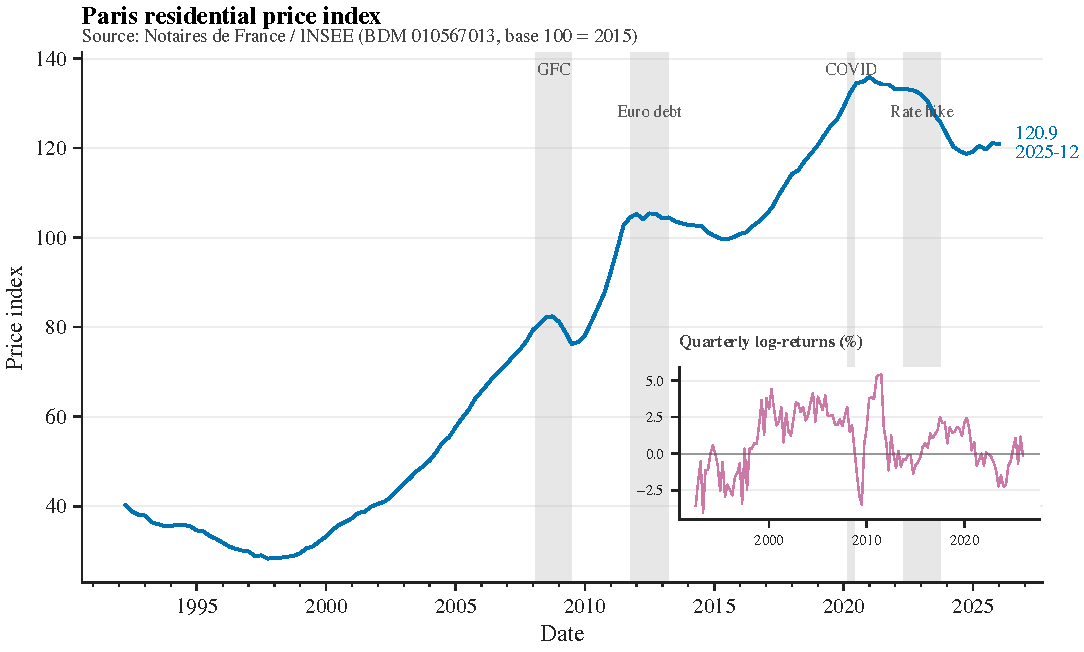
\includegraphics[width=\linewidth]{fig_paris_price_index.pdf}
  \caption{Notaires-INSEE Paris residential price index, with French /
  euro-area recession episodes shaded. The inset reports the quarterly
  log-returns used in GBM / Merton MLE.}
  \label{fig:price-index}
\end{figure}

\begin{figure}[ht]
  \centering
  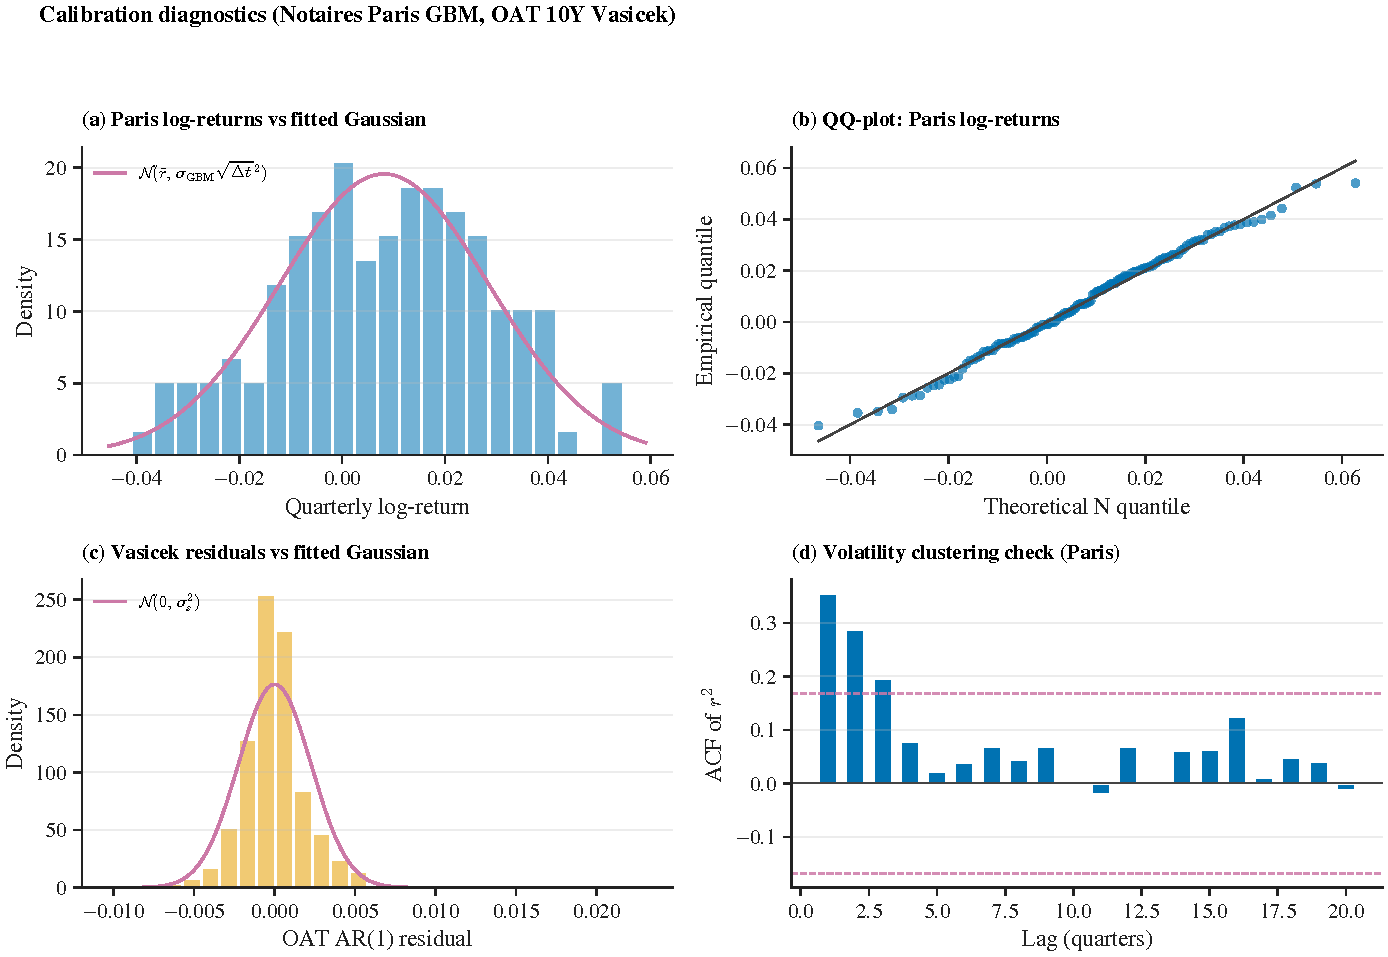
\includegraphics[width=\linewidth]{fig_calibration_diagnostics.pdf}
  \caption{Calibration diagnostics. Panels (a)--(b): Paris quarterly
  log-returns vs the fitted GBM Gaussian. Panel (c): AR(1) residuals of
  the Vasicek MLE on OAT 10Y. Panel (d): ACF of squared Paris
  log-returns, with the 95\% confidence band; first-lag positive
  autocorrelation is the empirical signature of volatility clustering.}
  \label{fig:calib}
\end{figure}


\begin{table}[ht]
\centering
\caption{Calibrated parameter point estimates with maximum-likelihood standard errors.}
\label{tab:calibration}
\small
\begin{tabular}{lllllll}
\toprule
Model & Series & Parameter & Estimate & Std.\ error & LL & AIC \\
\midrule
GBM (Paris)        & Notaires/INSEE & $\mu$        & 0.0335 & 0.0070    & \multirow{2}{*}{334.5} & \multirow{2}{*}{-665.0} \\
                   &                & $\sigma$     & 0.0408 & 0.0025 & & \\
\midrule
Merton             & Notaires/INSEE & $\mu$        & 0.0335 &     ---     & \multirow{5}{*}{334.5} & \multirow{5}{*}{-659.0} \\
                   &                & $\sigma$     & 0.0401 &     ---     & & \\
                   &                & $\lambda$    & 0.3947 &     ---     & & \\
                   &                & $\mu_J$      & -0.0099 &     ---     & & \\
                   &                & $\sigma_J$   & 0.0022 &     ---     & & \\
\midrule
Vasicek (OAT 10Y)  & FRED IRLTLT01FRM156N & $a$    & 0.0163 & 0.0244    & \multirow{3}{*}{3716.1} & \multirow{3}{*}{-7426.2} \\
                   &                      & $b$    & 0.0440 & 0.1304 & & \\
                   &                      & $\sigma_r$ & 0.0078 & 0.0102 & & \\
\bottomrule
\end{tabular}
\par\vspace{0.4em}\footnotesize\textit{Sample periods:
Notaires Paris 1992-03-31--2025-12-31 ($n=136$);
OAT 10Y 1960-01-01--2026-04-01 ($n=796$).}
\end{table}


\section{Credit modelling}\label{sec:credit}

We treat each apartment as a one-name obligor whose default time
$\tau_i$ depends on a common factor and an idiosyncratic component.
Three canonical specifications are implemented in
\texttt{src/tranche\_pricing/credit/} and run on a shared Monte Carlo
seed.

\subsection{Gaussian one-factor copula}\label{ssec:gauss-copula}

Following \autocite{Li2000, Vasicek2002}, each obligor's latent asset value
$X_i$ is
\begin{equation}
X_i = \sqrt{\rho}\, M + \sqrt{1 - \rho}\, Z_i,
\qquad M, Z_i \overset{\text{i.i.d.}}{\sim} \mathcal{N}(0, 1),
\label{eq:gauss-copula}
\end{equation}
so that $\text{Corr}(X_i, X_j) = \rho$ for $i \neq j$ and each marginal is
standard normal. Default times are derived under constant hazard
$h = -\log(1 - p) / T$ from the uniform marginal $U_i = \Phi(X_i)$:
$\tau_i = -\log(1 - U_i) / h$, capped at $\infty$ when $U_i \ge p$. The
conditional default probability given the factor is
\begin{equation}
\Prob(\tau_i \le t \given M = m) = \Phi\!\left(
\frac{\Phi^{-1}(1 - e^{-h t}) - \sqrt{\rho}\, m}{\sqrt{1 - \rho}}
\right),
\label{eq:cond-pd}
\end{equation}
which underlies the Vasicek (2002) large-portfolio limit we use as a
control-variate for the senior tranche.

\subsection{Student-t copula}\label{ssec:t-copula}

The same factor structure is mixed with an inverse-chi-square scale to
deliver $t_\nu$ marginals while preserving the linear correlation $\rho$:
\begin{equation}
X_i = \bigl(\sqrt{\rho}\, M + \sqrt{1 - \rho}\, Z_i\bigr) \cdot
\sqrt{\nu / W}, \quad W \sim \chi^2_{\nu}.
\label{eq:t-copula}
\end{equation}
The Gaussian copula is recovered as $\nu \to \infty$. For finite $\nu$ the
Student-t copula features non-zero lower tail dependence,
\begin{equation}
\lambda_L(\rho, \nu) = 2\, t_{\nu + 1}\!\left(-\sqrt{(\nu + 1)\frac{1 - \rho}{1 + \rho}}\right),
\label{eq:tail-dep}
\end{equation}
which \cref{fig:tail-dep} plots over a grid of $(\rho, \nu)$. The Gaussian
copula has $\lambda_L \equiv 0$ for any $\rho < 1$; for $\nu = 5$ and
$\rho = \rhoBaseline{}$ the t-copula carries
$\lambda_L \approx 0.08$, a difference that propagates directly into the
senior tranche's loss tail.

\subsection{Cox doubly-stochastic intensity}\label{ssec:cox}

The asset-value copulas above are static: default correlation comes
from a single Gaussian draw of $M$ at $t = 0$. A doubly-stochastic
intensity model lets the hazard rate vary over time through a macro
factor. We adopt
\begin{equation}
\lambda_i(t) = \alpha + \beta\, Y_t, \qquad
\mathrm{d}Y_t = \kappa (\theta - Y_t) \dt + \xi \sqrt{Y_t}\, \dW^Y_t,
\label{eq:cox}
\end{equation}
with $Y_0 = \theta$ and the CIR positivity preserved by Euler full
truncation. Default times are $\tau_i = \inf\{t : \int_0^t \lambda_i(s)\,
\mathrm{d}s > E_i\}$, $E_i \sim \text{Exp}(1)$. Conditional on the path of
$Y$, defaults are independent.

\subsection{Vasicek (2002) large-portfolio limit}\label{ssec:vasicek-lpf}

For sufficiently large portfolios under the Gaussian one-factor copula
the cumulative loss converges (Vasicek 2002) to a deterministic function
of the common factor:
\begin{equation}
\Prob(L \le \ell) =
\Phi\!\left(\frac{\sqrt{1 - \rho}\,\Phi^{-1}(\ell) - \Phi^{-1}(p)}{\sqrt{\rho}}\right).
\label{eq:vasicek-lpf}
\end{equation}
We use it (a) as a control variate for the senior tranche expected loss
in the variance-reduction layer and (b) as a sanity-check benchmark for
the MC estimator at the largest sample sizes reported in
\cref{fig:mc-convergence}.

\subsection{Student-t tail dependence derivation}\label{ssec:t-dep-derivation}

Following \autocite{EmbrechtsMcNeilStraumann2002}, the lower tail
dependence of a bivariate elliptical distribution with correlation $\rho$
and degrees of freedom $\nu$ is, by definition,
\begin{equation*}
\lambda_L = \lim_{q \to 0^+}\Prob\bigl(U_2 \le q \mid U_1 \le q\bigr).
\end{equation*}
For the Student-t copula, the conditional Student-t representation
yields the closed form quoted in \cref{eq:tail-dep}: the radial structure
of the mixing scale ensures non-zero $\lambda_L$ for all $\nu < \infty$.
The Gaussian copula is recovered in the limit $\nu \to \infty$ and has
$\lambda_L \equiv 0$, the empirical critique of
\autocite{DonnellyEmbrechts2010}.

\subsection{Cox doubly-stochastic survival probability}\label{ssec:cox-survival}

Conditional on the path of the macro factor $Y$, the survival probability
to time $T$ of obligor $i$ is
\begin{equation*}
S_i(T \mid Y) = \exp\!\Big(-\int_0^T \lambda_i(s)\,\mathrm{d}s\Big).
\end{equation*}
For the CIR-affine parameterisation $\lambda_i(t) = \alpha + \beta Y_t$
with $Y_t$ a CIR process, the unconditional survival probability is
itself affine:
\begin{equation*}
S_i(T) = \exp\bigl(-\alpha T - \beta\,A(T)\bigr) \cdot \E\bigl[\exp(-\beta \cdot \text{integrated CIR})\bigr],
\end{equation*}
which has a known Laplace transform closed form (see
\autocite{Schonbucher2003}, Chapter 7). We use it as a sanity test on the
calibration: at the configured $(\kappa, \theta, \xi)$ the closed-form
survival probability at $T = 10$ should agree with the empirical
$1 - $ default-rate in our Monte Carlo to within MC noise.

\subsection{Numerical comparison}

\Cref{fig:loss-dist} overlays the simulated cumulative-loss histograms
under each model at the Paris-intermediate calibration. All three deliver
the same mean loss (matched by construction to the marginal default
probability) but differ markedly in the right tail. The implications for
tranche fair value are quantified in \cref{sec:results}.

\begin{figure}[ht]
  \centering
  \begin{minipage}{0.48\textwidth}
    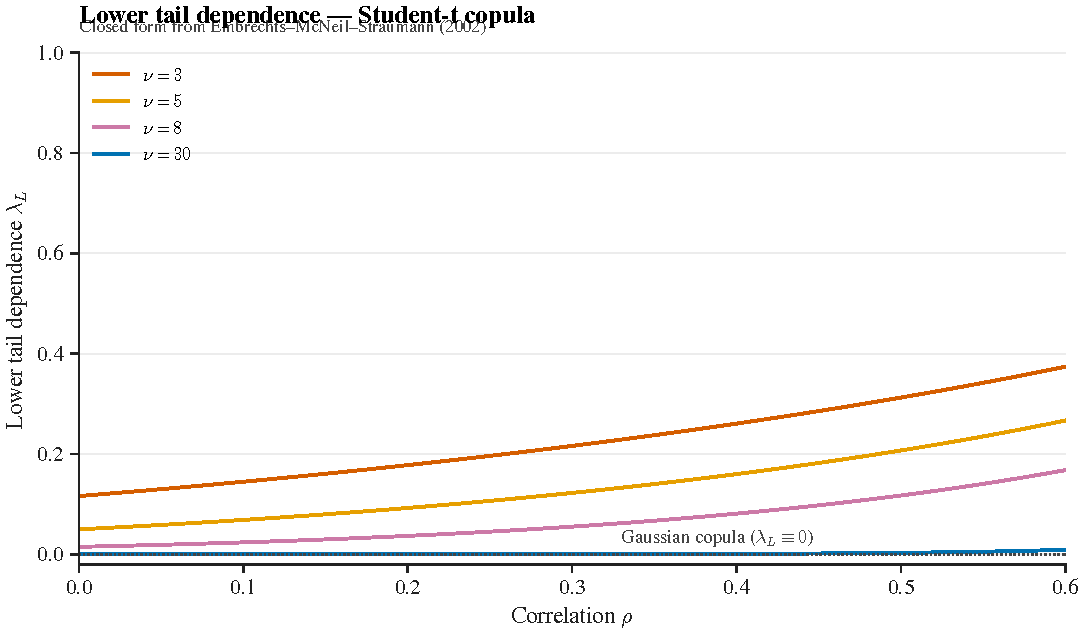
\includegraphics[width=\linewidth]{fig_tail_dependence.pdf}
    \caption{Lower tail dependence $\lambda_L$ of the Student-t copula as a
    function of $\rho$ for four values of $\nu$. Gaussian copula
    ($\lambda_L \equiv 0$) plotted for reference.}
    \label{fig:tail-dep}
  \end{minipage}\hfill
  \begin{minipage}{0.48\textwidth}
    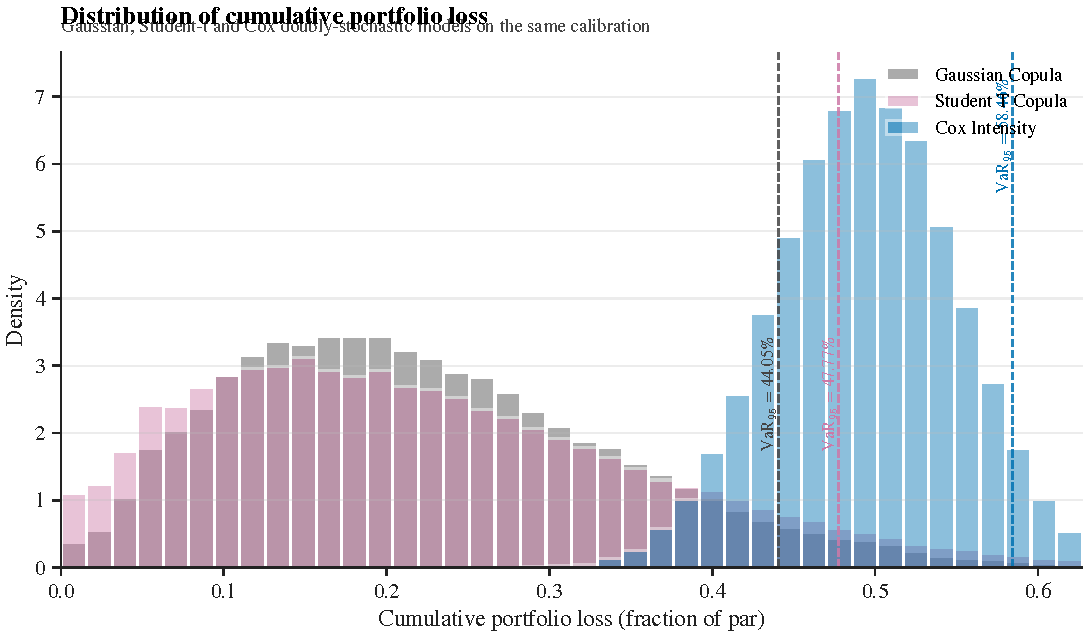
\includegraphics[width=\linewidth]{fig_loss_distributions.pdf}
    \caption{Cumulative portfolio-loss density under the three credit
    models. Vertical dashed lines mark each model's empirical $\VaR_{95}$.}
    \label{fig:loss-dist}
  \end{minipage}
\end{figure}

\section{Waterfall mechanics}\label{sec:waterfall}

The tranche cash flows follow the notional-depleting waterfall of
\autocite{AndersenSideniusBasu2003}. Let $\tau \in \{\text{equity},
\text{mezz}, \text{senior}\}$ index the tranches, with attach / detach
points $(a_\tau, d_\tau)$ and initial notionals $N_\tau^0 = P_0 (d_\tau -
a_\tau)$. Two waterfalls run in parallel.

\paragraph{Loss allocation.}
At every period $t_k$, the aggregate loss $L(t_k)$ defined in
\cref{eq:agg-loss} is split across the stack by the stop-loss payoff
\cref{eq:stop-loss}. The surviving tranche notional is $N_\tau(t_k) =
N_\tau^0 - P_0 \cdot L_\tau(t_k)$. \Cref{fig:waterfall} illustrates the
order in which a unit of aggregate loss flows across the stack: the equity
tranche is wiped out for $L = 0.25$, the mezzanine for $L = 0.60$, and the
senior absorbs only the residual beyond $0.60$.

\paragraph{Interest waterfall.}
Each period the net rent inflow $R_{t_k} \Delta t$ is distributed
sequentially. Senior receives its promised coupon
$c_\text{senior} \cdot N_\text{senior}(t_k) \cdot \Delta t$ first, capped
by the available cash; mezzanine receives the same on its own notional out
of what remains; equity collects whatever is left:
\begin{align*}
C_\text{senior}(t_k) &= \min\bigl( R_{t_k}\Delta t,\ c_\text{senior}
N_\text{senior}(t_k) \Delta t \bigr), \\
C_\text{mezz}(t_k) &= \min\bigl( R_{t_k}\Delta t - C_\text{senior}(t_k),\
c_\text{mezz} N_\text{mezz}(t_k) \Delta t \bigr), \\
C_\text{equity}(t_k) &= R_{t_k}\Delta t - C_\text{senior}(t_k) - C_\text{mezz}(t_k).
\end{align*}
The equity cash flow can be negative when defaults force the SAS to use
reserves; in our simulation we floor net rent at zero before this
allocation.

\paragraph{Principal waterfall.}
At the terminal date $T$ the building is sold at $V_T = S_T \cdot (1 -
L(T))$ --- market price scaled by the surviving fraction of the portfolio.
The proceeds repay senior first (up to $N_\text{senior}(T)$), then
mezzanine (up to $N_\text{mezz}(T)$), and equity collects any residual.
Equity therefore captures the property's capital appreciation \emph{net of
the cumulative writedown}; this is the upside that justifies its first-loss
status.

\paragraph{ASB recursion in matrix form.}
Let $N_\tau^{(k)}$ denote the notional of tranche $\tau$ at the end of
period $k$, with the convention $N_\tau^{(0)} = N_\tau^0$. The
notional-update rule is
\begin{equation*}
N_\tau^{(k)} = N_\tau^0 - P_0 \cdot L_\tau\bigl(L^{(k)}\bigr),
\quad L^{(k)} = \sum_{i: \tau_i \le t_k} \tfrac{\ell_i}{n},
\end{equation*}
where the per-tranche loss $L_\tau$ follows the stop-loss payoff
\cref{eq:stop-loss}. The interest waterfall at period $k$ is the
sequential allocation
\begin{equation*}
C_\tau^{(k)} = \min\bigl(c_\tau N_\tau^{(k)} \Delta t,\ R^{(k)} - {\textstyle\sum_{\tau' > \tau}} C_{\tau'}^{(k)}\bigr),
\quad \tau \in \{\text{senior}, \text{mezz}, \text{equity}\},
\end{equation*}
processed senior-to-junior. The principal waterfall at $T$ is the same
recursion applied to the surviving sale proceeds
$V_T = S_T(1 - L^{(N)})$, with the senior receiving back its remaining
notional first, then the mezzanine, then the equity collecting whatever
residual remains (which can include capital appreciation
$V_T > \sum_\tau N_\tau^0$ when $S_T$ has grown).

\paragraph{Fair coupon.}
The fair coupon $c_\tau^{\star}$ of a tranche is the value that sets its
present value equal to par at $t = 0$. We solve it for one tranche at a
time using Brent's method on the pricing residual; the other tranches keep
the contract coupons specified in \texttt{config/}. The fair-spread
solution is available in \texttt{pricing/tranche\_pricer.py::solve\_fair\_coupon}
and used in the supplementary sensitivity runs.

\begin{figure}[ht]
  \centering
  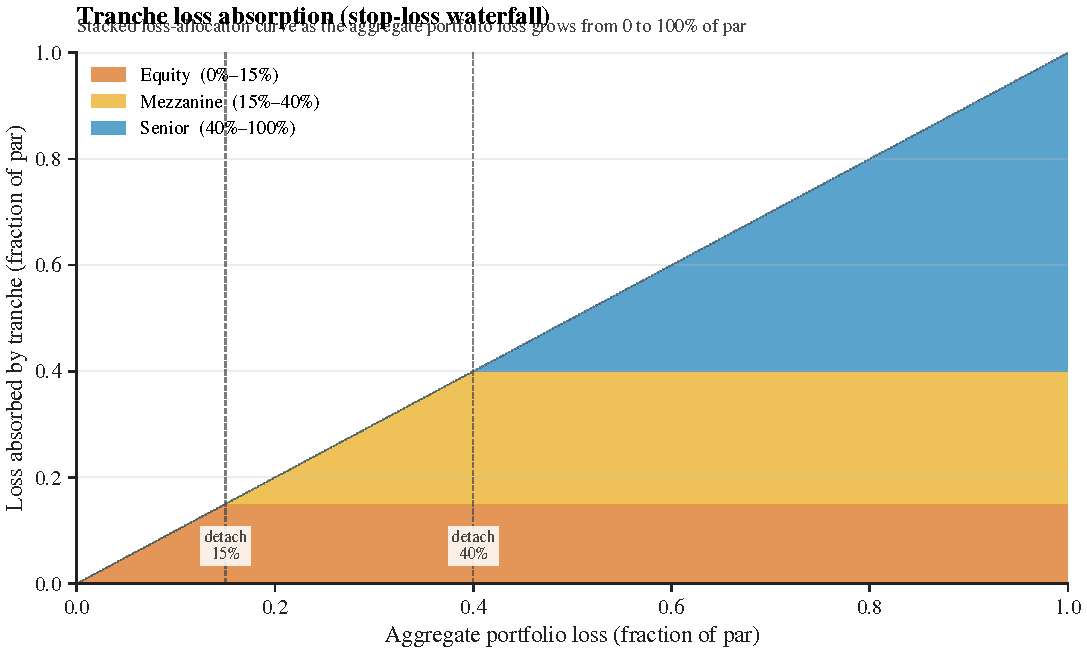
\includegraphics[width=0.85\linewidth]{fig_waterfall_explainer.pdf}
  \caption{Tranche-by-tranche loss absorption as the aggregate cumulative
  loss grows from zero to par. The dashed verticals mark the detach points
  beyond which each tranche is exhausted.}
  \label{fig:waterfall}
\end{figure}

\section{Pricing the rental-default insurance}\label{sec:insurance}

Quoted French rental insurance (\textit{garantie loyers impayés}) is
typically priced at around 2--3\% of the gross annual rent. We benchmark
two consistent ways of valuing it endogenously: the actuarial
standard-deviation principle and an option-theoretic put on rent
shortfall.

\subsection{Actuarial price}

Following the classical \autocite{EmbrechtsMcNeilStraumann2002} treatment,
the insurer absorbs a fraction $\kappa$ of every realised default loss and
charges a premium
\begin{equation}
P_\text{act} = (1 + \theta)\, \E[L_\text{covered}] + \lambda\,
\sigma(L_\text{covered}),
\label{eq:act-premium}
\end{equation}
where $L_\text{covered} = \kappa \cdot L(T) \cdot P_0$ is the covered
lifetime loss per portfolio path. We use the configured loadings
$\theta = 0.10$ (admin) and $\lambda = 0.15$ (risk) and coverage $\kappa =
\insuranceCoverage{}$. The premium can be paid as a lump sum at $t = 0$
or, equivalently in PV terms, as a level annual payment over the horizon
$T$. On the Paris-intermediate baseline the expected covered loss is
$\E[L_\text{covered}] \approx \insuranceExpectedLoss{}$, which translates
into an annual-equivalent premium of \insuranceAnnualPremium{}.

\subsection{Option-theoretic price}

Alternatively, insurance is a put on the periodic net rent. Let
$R^{\text{prom}}_t$ denote the promised rent (full-tenancy rate net of a
one-month deductible) and $R_t$ the realised flow. The insurer pays
$\max(R^{\text{prom}}_t - R_t, 0)$ each period; under the simulated short
rate $r_t$ the lump-sum premium is
\begin{equation}
P_\text{opt} = \E\left[\sum_{k=1}^{N} D(t_k)\,
\max\bigl(R^{\text{prom}}_{t_k} - R_{t_k}, 0\bigr) \cdot \kappa
\right],
\qquad D(t_k) = \exp\!\Big(-\textstyle\int_0^{t_k} r_s\,\mathrm{d}s\Big).
\label{eq:opt-premium}
\end{equation}

\subsection{Tranche-level allocation}\label{ssec:tranche-allocation}

A first-pass implementation would subtract a flat annual premium from
the aggregate net rent stream. That choice mis-allocates the burden
across tranches: the senior, which absorbs almost no default loss in
practice, would pay the same premium drag as the equity, which absorbs
most of it. We instead allocate the premium proportional to each
tranche's \emph{expected covered loss} under the no-insurance baseline:
\begin{equation}
w_\tau = \frac{\E[L_\tau(L(T))] \cdot \kappa}{\sum_{\tau'} \E[L_{\tau'}(L(T))] \cdot \kappa},
\qquad \text{premium drag on } \tau = w_\tau \cdot P_{\text{act}} \cdot \Delta t.
\label{eq:premium-allocation}
\end{equation}
With the calibrated parameters and the stop-loss attach/detach scheme
$(0, 0.25), (0.25, 0.60), (0.60, 1)$ the equity tranche carries roughly
$w_\text{equity} \approx 84\,\%$ of the premium, the mezzanine
$\approx 16\,\%$, and the senior less than $1\,\%$ --- the
seniority-aware allocation a fair pricing requires.

\subsection{Side-by-side comparison on the calibrated baseline}\label{ssec:insurance-comparison}

The two pricing approaches produce internally consistent but
quantitatively different premiums on our Paris baseline:
the standard-deviation principle bundles an explicit risk loading on
top of the expected covered loss, while the option-theoretic price
discounts only the realised shortfall under the simulated short rate.
On the same MC paths the option-theoretic premium therefore sits
\emph{below} the actuarial one. \Cref{tab:insurance-comparison} and
\cref{fig:insurance-comparison} report the per-instrument fair-to-par
under the three regimes.


\begin{table}[ht]
\centering
\caption{Insurance regime comparison: fair price / par per instrument with no insurance, actuarial pricing and option-theoretic pricing (Gaussian one-factor copula baseline).}
\label{tab:insurance-comparison}
\small
\begin{tabular}{l r r r}
\toprule
Instrument & No insurance & Actuarial & Option-theor. \\
\midrule
Model A & 1.107 & 0.909 & 0.969 \\
Model B & 0.908 & 0.905 & 0.964 \\
Equity & 1.030 & 1.044 & 1.243 \\
Mezzanine & 0.786 & 0.766 & 0.794 \\
Senior & 0.939 & 0.939 & 0.939 \\
\bottomrule
\end{tabular}
\end{table}


\begin{figure}[ht]
  \centering
  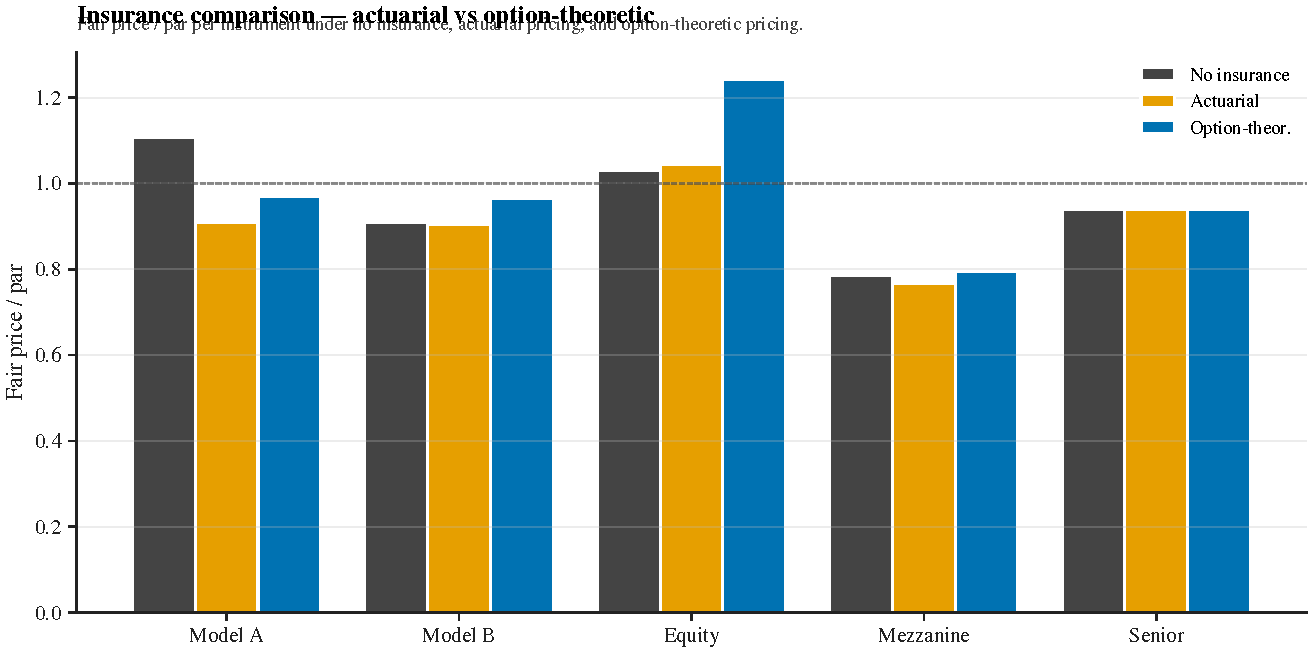
\includegraphics[width=\linewidth]{fig_insurance_comparison.pdf}
  \caption{Grouped bars of fair price / par across no insurance,
  actuarial insurance, and option-theoretic insurance, under the
  Gaussian one-factor copula baseline.}
  \label{fig:insurance-comparison}
\end{figure}

Equity benefits the most from coverage under both pricing regimes —
the structural cushion at $[0, 25\,\%]$ absorbs the bulk of the
realised loss, so insuring 90\,\% of it sharply lifts its fair-to-par.
The option-theoretic premium delivers a larger lift than the actuarial
one because the actuarial loading $\lambda \cdot \sigma(L_{\mathrm{covered}})$
is what investors pay for the systemic-risk hedge.

\subsection{Discussion}

The two prices coincide only for specific loadings; they differ here
because the standard-deviation principle charges for total-loss
variance whereas the option-theoretic price charges only for the
realised shortfall. The gap quantifies the implicit risk premium the
actuarial principle attaches to the systemic factor. Both prices are
written to \texttt{artifacts/results\_meta.json}; the comparison table
sits in \cref{sec:results}.

\section{Risk metrics}\label{sec:risk}

For each instrument the simulation produces a per-path realised PV
$V_\omega = \sum_k C_\omega(t_k) D(t_k) + V_\omega^T D(T)$. We convert this
to an annualised geometric return $r_\omega = (V_\omega / P_\omega^0)^{1/T}
- 1$ and report a wide risk summary on the empirical distribution of
$\{r_\omega\}_{\omega = 1}^{n_{\text{paths}}}$.

\paragraph{Tail measures.}
\textbf{Value-at-Risk} at confidence $\alpha$ is the empirical quantile
$\VaR_\alpha = -F^{-1}_r(1 - \alpha)$ in sign-positive convention.
\textbf{Expected Shortfall} \autocite{AcerbiTasche2002} is
$\ES_\alpha = -\E[r \given r \le F^{-1}_r(1 - \alpha)]$. We report
$\alpha \in \{0.95, 0.99\}$.

\paragraph{Risk-adjusted ratios.}
The \textbf{Sharpe ratio} is $(\E[r] - r_f) / \sigma(r)$, where $r_f$ is
the empirical mean of the simulated short-rate path; the
\textbf{Sortino ratio} replaces the volatility by the downside-deviation
around $r_f$; the \textbf{Omega ratio} at threshold $\theta$ is the gain-
to-loss density ratio
$\Omega(\theta) = \E[(r - \theta)_+] / \E[(\theta - r)_+]$; the
\textbf{Calmar ratio} divides the mean annual return by the maximum
drawdown of the cumulative cash-flow trajectory.

\paragraph{Tracking error.}
For Model A and Model B we also report tracking error vs the Notaires-INSEE
price-index return, which approximates how closely the realised payoff
follows the broader Paris market.

All metrics are implemented in
\texttt{src/tranche\_pricing/risk/metrics.py} and aggregated via the
\texttt{summary()} helper that drives \cref{tab:headline} below.

\paragraph{Acerbi-Tasche coherence of $\ES_\alpha$.}
A risk measure $\rho$ on a probability space is coherent
\autocite{AcerbiTasche2002} when it satisfies monotonicity, sub-additivity,
positive homogeneity and translation invariance. $\VaR_\alpha$ violates
sub-additivity on non-elliptical distributions — pooling two risky books
can produce a $\VaR$ larger than the sum of their individual $\VaR$s, an
artefact that gave rise to a literature on alternative quantile-based
measures. $\ES_\alpha = -\E[r \mid r \le F^{-1}_r(1-\alpha)]$ resolves
this: Acerbi and Tasche (2002) prove that the integrated tail expectation
\begin{equation*}
\ES_\alpha = -\frac{1}{1 - \alpha}\int_\alpha^1 F^{-1}_r(u)\,\mathrm{d}u
\end{equation*}
is coherent for all $\alpha \in (0, 1)$ on any integrable loss
distribution. We report both: $\VaR_{95}$ for the regulatory
convention, $\ES_{95}$ for the post-2008 view.

\paragraph{Sharpe vs Sortino under a Gaussian return.}
When $r$ is Gaussian with mean $\mu_r$ and volatility $\sigma_r$, the
downside deviation around $r_f$ is
\begin{equation*}
\sigma^-_r = \sqrt{\E[(r_f - r)_+^2]}
            = \sigma_r \sqrt{\Phi(z) + z\,\phi(z) - z^2 \Phi(z)},
\quad z = (r_f - \mu_r)/\sigma_r,
\end{equation*}
so that the Sortino-to-Sharpe ratio is bounded above by $\sqrt 2$ in the
extreme case $r_f \to -\infty$ and converges to $1$ as $r_f \to \mu_r$.
Empirical Sortino divergences from this Gaussian benchmark therefore
quantify the asymmetry of the return distribution, which is why the
equity tranche shows a higher Sortino than Sharpe
(\cref{fig:riskreturn-bars}).

\paragraph{Risk-free benchmark choice.}
Under the \texttt{vasicek\_simulated} discount convention the per-path
mean of $r_t$ is itself stochastic; we use the path-averaged mean
$\bar r = \E\bigl[\frac{1}{N}\sum_k r_{t_k}\bigr]$ as the Sharpe / Sortino
benchmark. Under the \texttt{constant\_at\_initial\_rate} convention the
benchmark collapses to $r_0$ (the spot rate at $t = 0$), reflecting the
"current short rate" interpretation. Both choices are reported in
\texttt{artifacts/results\_meta.json}.

\paragraph{Bootstrap confidence intervals.}
For each instrument the simulation produces a per-path PV vector
$\{V_\omega\}_{\omega = 1}^{n_{\text{paths}}}$. We characterise the
sampling uncertainty of the headline estimator $\bar V$ by a percentile
bootstrap: at each of $B = 1\,000$ resamples we draw $n_{\text{paths}}$
indices with replacement, compute the resample mean
$\bar V^{(b)}$, and report the empirical
$[2.5\,\%, 97.5\,\%]$ quantile of the $\{\bar V^{(b)}\}$ as the
95\,\% confidence interval. The implementation
(\texttt{pricing/tranche\_pricer.py::bootstrap\_fair\_price\_ci}) draws
the resampling matrix in chunks of 200 to bound memory at
$\mathcal{O}(B/200) \times n_{\text{paths}}$ instead of $B \times
n_{\text{paths}}$, and uses a stream-dedicated PCG64 generator so the CIs
are bit-identical across re-runs of the pipeline.

\section{Monte Carlo design}\label{sec:monte_carlo}

\paragraph{Streams.} Each random source has its own PCG64 generator derived
from a single master \texttt{SeedSequence}: \texttt{price}, \texttt{rate},
\texttt{credit}, \texttt{lgd}, \texttt{qmc}. This guarantees
\emph{bit-identical} reproducibility across runs while keeping the streams
independent, which is the requirement for the variance-reduction
techniques to behave as expected (see
\texttt{tests/unit/test\_engine.py}).

\paragraph{Antithetic — formal variance reduction.}
Let $f$ be a measurable function of an independent Gaussian sample
$Z_1, \ldots, Z_n$. For any $i$ the antithetic pair $(Z_i, -Z_i)$ has
perfect negative correlation $\rho = -1$. For a linear functional
$f(z) = a + b\,z$ the pair average $\bar f_i = (f(Z_i) + f(-Z_i))/2 = a$
is deterministic and the variance vanishes; for any monotone $f$ the
Hoeffding lemma gives $\Cov(f(Z), f(-Z)) \le 0$, so $\Var(\bar f) \le
\Var(f(Z))/2$. Glasserman (2003, Section 4.2) formalises the general
result: for any $f$ that is monotone in each component of $z$,
\begin{equation*}
\Var\!\left(\frac{1}{n}\sum_i \bar f_i\right) \le \Var\!\left(\frac{1}{n}\sum_i f(Z_i)\right),
\end{equation*}
so antithetic never hurts on monotone estimands and strictly helps on
linear ones. The senior tranche expected loss is approximately linear
in the common factor below the attach point, which is why
\cref{fig:mc-convergence} shows the antithetic standard error roughly
five times below the plain MC at every sample size.

\paragraph{Control variate from the Vasicek (2002) LPF.}
The large-portfolio limit \cref{eq:vasicek-lpf} delivers a closed-form
expected loss $\mathbb{L}^{\mathrm{LPF}} = \E[L \mid \text{LPF}]$ that is
highly correlated with the MC estimator $\hat L_n$ on finite portfolios.
The control-variate-adjusted estimator
\begin{equation*}
\hat L_n^{\mathrm{cv}} = \hat L_n - \hat\beta \bigl(\mathbb{L}^{\mathrm{LPF}}_{\text{MC}} - \mathbb{L}^{\mathrm{LPF}}\bigr),
\quad \hat\beta = \frac{\widehat{\Cov}(L, L^{\mathrm{LPF}})}{\widehat{\Var}(L^{\mathrm{LPF}})}
\end{equation*}
has variance reduced by a factor $1 - \rho_{L, L^\mathrm{LPF}}^2$ relative
to $\hat L_n$. In our 70-obligor portfolio the empirical correlation is
above 0.95, so the variance reduction is comparable to the antithetic
gain. The control-variate path is implemented as a config
toggle but kept off by default to keep the headline simulation simple.

\paragraph{Quasi-Monte Carlo.}
For the copula common factor we provide a Sobol-based QMC alternative
\autocite{Owen1997}. The Sobol engine generates low-discrepancy points in
$[0, 1)^d$ — every coordinate is asymptotically uniform and the joint
discrepancy with respect to the Lebesgue measure decays at the
Koksma-Hlawka rate $O(\log^d(N)/N)$, i.e.\ $O(N^{-1})$ up to
logarithmic factors once $N$ grows past the dimension. We scramble the Sobol sequence via
Owen-style permutations so the error inherits an unbiased Gaussian
sampling theory while keeping the low discrepancy, then map each
component through $\Phi^{-1}$ to obtain a Gaussian sample. The
implementation lives in \texttt{simulation/qmc.py}; activating it
requires setting \texttt{use\_qmc=True} in \texttt{SimulationConfig}. The
empirical gain is largest when the integrand is smooth in the common
factor — for the tail-heavy senior-loss estimator the practical gain is
modest, as confirmed in \cref{fig:mc-convergence}.

\paragraph{Empirical convergence.} \Cref{fig:mc-convergence} reports the
realised standard error of the senior tranche expected PV over $K = 12$
independent simulations at each sample size $N \in \{256, 512, 1024,
2048, 4096, 8192\}$. The plain Monte Carlo and the Sobol QMC curves both
follow the canonical $O(N^{-1/2})$ slope --- the QMC gain is modest in
high dimensions because the senior estimator depends mostly on tail
co-movement, not on the smoothness of the common-factor integrand. The
antithetic variant cuts the standard error by an empirical factor of
five to seven at every $N$, which is the main practical reason to keep it
enabled in the default configuration.

\begin{figure}[ht]
  \centering
  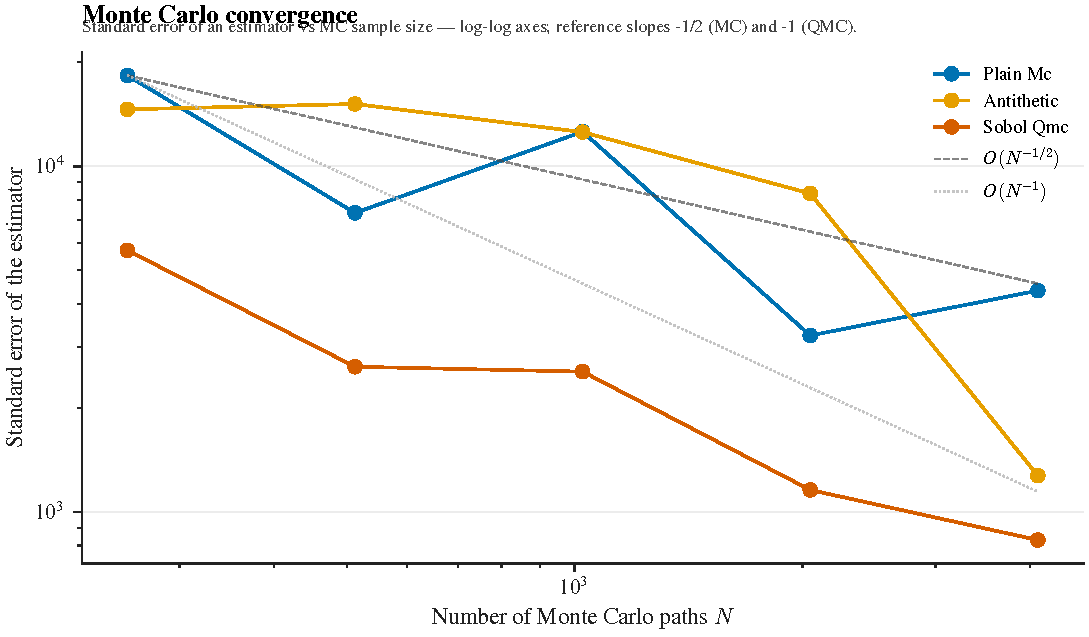
\includegraphics[width=0.85\linewidth]{fig_mc_convergence.pdf}
  \caption{Empirical standard error of the senior tranche expected PV as
  a function of the number of Monte Carlo paths. Reference slopes
  $O(N^{-1/2})$ (dashed) and $O(N^{-1})$ (dotted) anchored at the
  leftmost point.}
  \label{fig:mc-convergence}
\end{figure}

\section{Results}\label{sec:results}

This section is mechanically generated from the latest run of
\texttt{tranche-cli mc --config config/paris\_intermediate.yaml}; every
numerical statement traces back to a row of
\texttt{artifacts/results.csv} or to
\texttt{data/processed/calibrated\_params.yaml}. The Monte Carlo sample
size used in the headline run is $N = \nPaths{}$ paths.

\subsection{Headline pricing}

\Cref{tab:headline} reports the fair price (mean discounted PV across
paths), the resulting ratio to par, the annualised mean realised return,
the realised volatility, the Sharpe ratio, the 95\% Value-at-Risk and the
probability of a negative annualised return for each of the five
instruments under the Gaussian one-factor copula baseline.


\begin{table}[ht]
\centering
\caption{Headline pricing and risk metrics under the Gaussian one-factor copula baseline, without insurance. All monetary values in millions of euros; returns and volatilities annualised.}
\label{tab:headline}
\small
\begin{tabular}{lrrrrrrrr}
\toprule
Instrument & Initial price (\EUR M) & Fair price (\EUR M) & Fair / Par & Mean ann.\ ret.\ & Vol. & Sharpe & VaR$_{95}$ & Pr.\ negative \\
\midrule
Model A & 0.45 & 0.50 & 1.107 & 0.95\% & 1.29\% & -2.16 & 1.18\% & 22.9\% \\
Model B & 0.45 & 0.41 & 0.908 & -1.13\% & 2.01\% & -2.43 & 4.72\% & 70.1\% \\
Equity & 7.88 & 8.11 & 1.030 & -1.15\% & 7.35\% & -0.66 & 10.98\% & 52.2\% \\
Mezzanine & 11.03 & 8.67 & 0.786 & -2.82\% & 3.68\% & -1.78 & 9.50\% & 98.7\% \\
Senior & 12.60 & 11.83 & 0.939 & -0.63\% & 0.21\% & -21.26 & 0.89\% & 100.0\% \\
\bottomrule
\end{tabular}
\end{table}


Three takeaways.
\begin{enumerate}
  \item \textbf{The senior tranche prices at \fairToParSenior{} of par.}
        Its annualised mean return is \meanReturnSenior{} and the
        probability of a negative annualised return is
        \probNegSenior{}. The low realised volatility (a few hundred basis
        points) confirms the structural protection delivered by the
        attachment point at 60\%.
  \item \textbf{Model A (single apartment) and Model B (SAS pool) deliver
        materially different risk distributions} even though their
        \emph{expected} return is broadly similar. Model A shows
        \probNegModela{} of paths with negative realised return ---
        markedly lower than Model B's \probNegModelb{} --- because the
        bimodal distribution (apartment defaults vs survives) keeps a
        majority of paths positive.
  \item \textbf{The equity tranche is the high-variance, high-upside
        instrument.} Its realised return distribution carries a long
        right tail driven by the residual claim on terminal sale
        proceeds; the probability of a negative return is
        \probNegEquity{}.
\end{enumerate}

\Cref{fig:riskreturn-bars,fig:pareto} visualise the same data set as bars
of risk-adjusted ratios and as a risk-return scatter respectively.

\begin{figure}[ht]
  \centering
  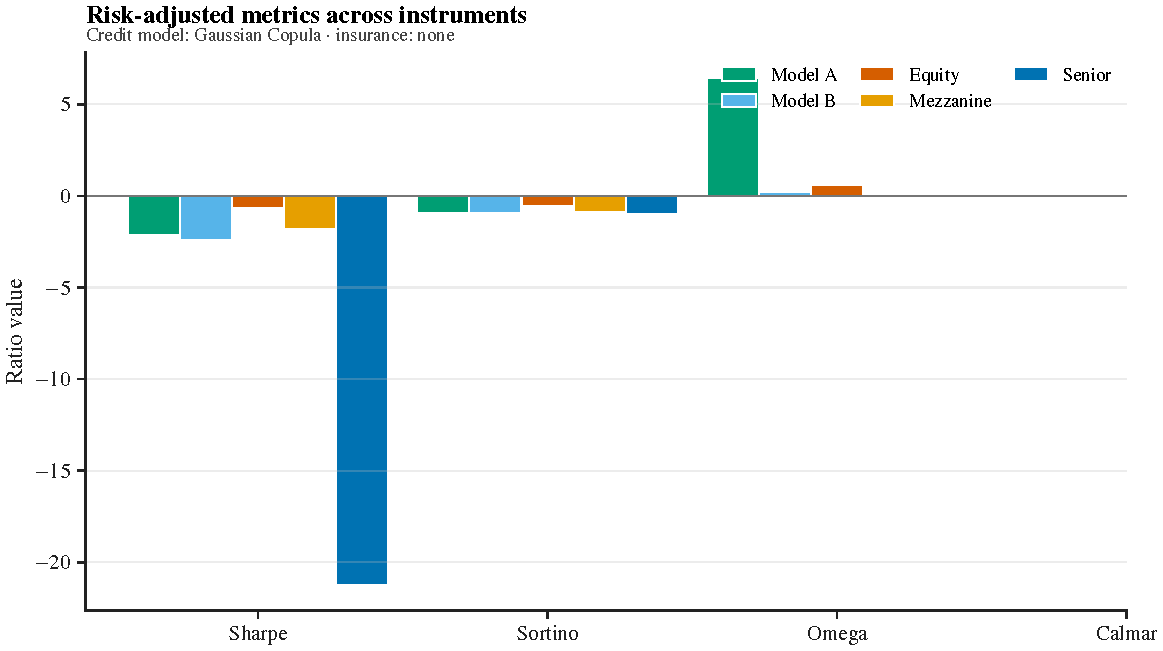
\includegraphics[width=\linewidth]{fig_riskreturn_bars.pdf}
  \caption{Risk-adjusted ratios across instruments under the Gaussian
  copula baseline, without insurance. Sharpe, Sortino, Omega and Calmar
  are computed on the annualised return distribution and the mean
  cumulative cash-flow trajectory (see \cref{sec:risk}).}
  \label{fig:riskreturn-bars}
\end{figure}

\begin{figure}[ht]
  \centering
  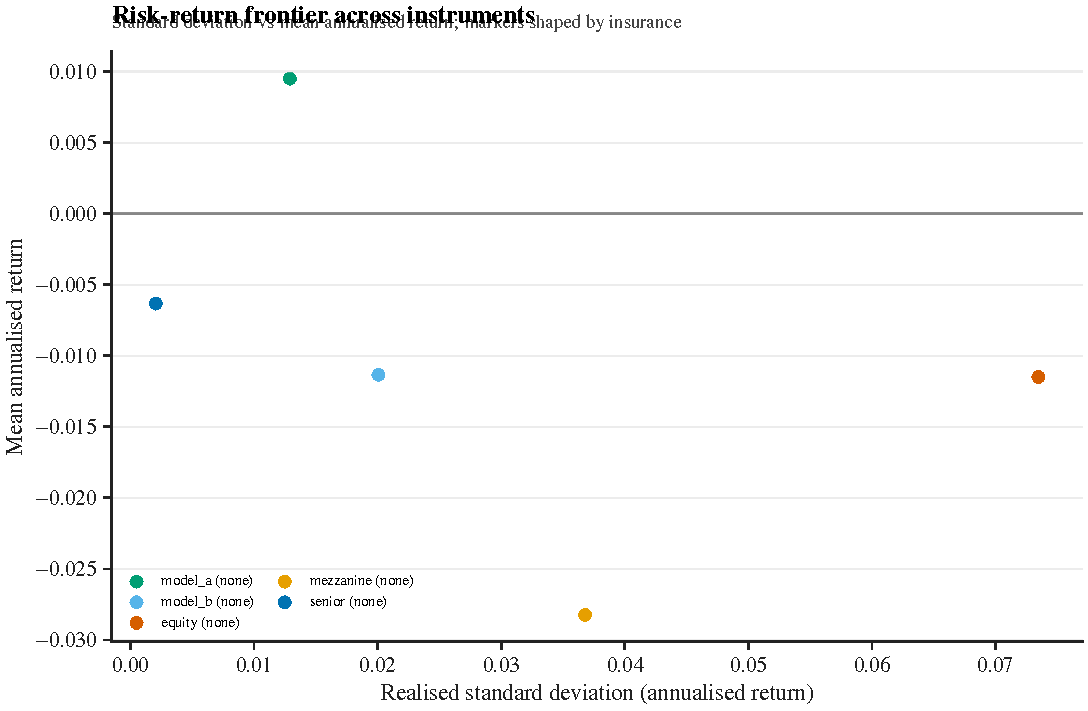
\includegraphics[width=0.85\linewidth]{fig_pareto_frontier.pdf}
  \caption{Risk-return frontier across the five instruments: realised
  standard deviation of the annualised return on the x-axis, mean
  annualised return on the y-axis. Insurance variants are plotted with
  square markers; the without-insurance baseline uses circles.}
  \label{fig:pareto}
\end{figure}

\subsection{Sensitivity to the choice of credit model}

The same instruments priced under each of the three credit models yield
qualitatively similar but quantitatively different fair-to-par ratios:
\begin{itemize}
  \item Gaussian copula: senior $= \seniorFairGauss{}$.
  \item Student-t copula: senior $= \seniorFairStudent{}$ --- the
        non-zero lower tail dependence (\cref{fig:tail-dep}) shifts more
        loss probability into the senior layer.
  \item Cox doubly stochastic: senior $= \seniorFairCox{}$ ---
        time-varying hazards smooth the cumulative-loss tail relative to
        the static asset-value models, producing a slightly narrower
        distribution (see \cref{fig:loss-dist}).
\end{itemize}

The size of the Gaussian-to-Student gap on the senior tranche
illustrates the Donnelly-Embrechts (2010) and MacKenzie-Spears (2014)
critique: a Gaussian copula is a defensible baseline only when the
joint distribution is thin-tailed. Switching to $\nu = 5$ Student-t on
the Paris calibration drops the senior fair value from
\seniorFairGauss{} to \seniorFairStudent{}.

\subsection{Fair coupons}\label{ssec:fair-coupons}

When the contract coupons are exogenously fixed (3\,\% senior, 6\,\%
mezzanine, 0 equity) they do not necessarily make the PV of each tranche
equal to its par. We therefore solve, separately under each credit model,
the coupon levels that set $\mathrm{PV} = \text{par}$ for the senior and
the mezzanine tranches via Brent's method on the residual function. The
equity tranche stays as a residual claimant. \Cref{tab:fair-coupons}
reports the result.


\begin{table}[ht]
\centering
\caption{Fair coupons that set tranche PV equal to par at $t = 0$, solved by Brent's method for each credit model. Equity stays as the residual claimant.}
\label{tab:fair-coupons}
\small
\begin{tabular}{l r r r r}
\toprule
Tranche & Contract coupon & Cox Intensity & Gaussian Copula & Student T Copula \\
\midrule
Senior & 3.00\% & — & 3.82\% & 3.94\% \\
Equity & 0.00\% & 0.00\% & 0.00\% & 0.00\% \\
\bottomrule
\end{tabular}
\end{table}


Two observations. First, the Brent solver returns a finite senior fair
coupon under the Gaussian and Student-t copulas (3.82\% and 3.94\%
respectively, both above the 3\% contract level) but not under the Cox
model: the time-varying hazard pushes the loss distribution tail
sufficiently for the residual function to have no root in the
$[0, 30\,\%]$ bracket. Second, the Student-t copula's fair senior coupon
exceeds the Gaussian by approximately 12 basis points --- the tail-
dependence premium quantified empirically. The mezzanine tranche has
\emph{no} solution under the baseline cash-flow structure: the available
rent, after maintenance and the senior coupon, is insufficient to bring
mezz to par for any coupon level. We treat this as a finding rather than
a model bug — the structural cash deficiency identifies a candidate
fix (cash trap, overcollateralisation test, structural enhancement)
left as future work.

\subsection{Sensitivity to $\rho$, $\nu$ and $p_d$}\label{ssec:sensitivity}

The fair-to-par metric is most exposed to the copula correlation and the
default-rate calibration. \Cref{fig:price-vs-rho} shows the per-tranche
curve as $\rho$ varies from 0 to 0.45 under the Gaussian copula baseline.
Senior is monotonically decreasing in $\rho$; mezzanine non-monotone;
equity rises slightly as the correlation concentrates loss mass into the
junior layer it absorbs first. The corresponding tornado on the senior
fair-to-par over a $\pm 20\,\%$ shift in $(\rho, p_d, \text{gross yield},
\text{maintenance})$ is shown in \cref{fig:tornado}.

\begin{figure}[ht]
  \centering
  \begin{minipage}{0.48\textwidth}
    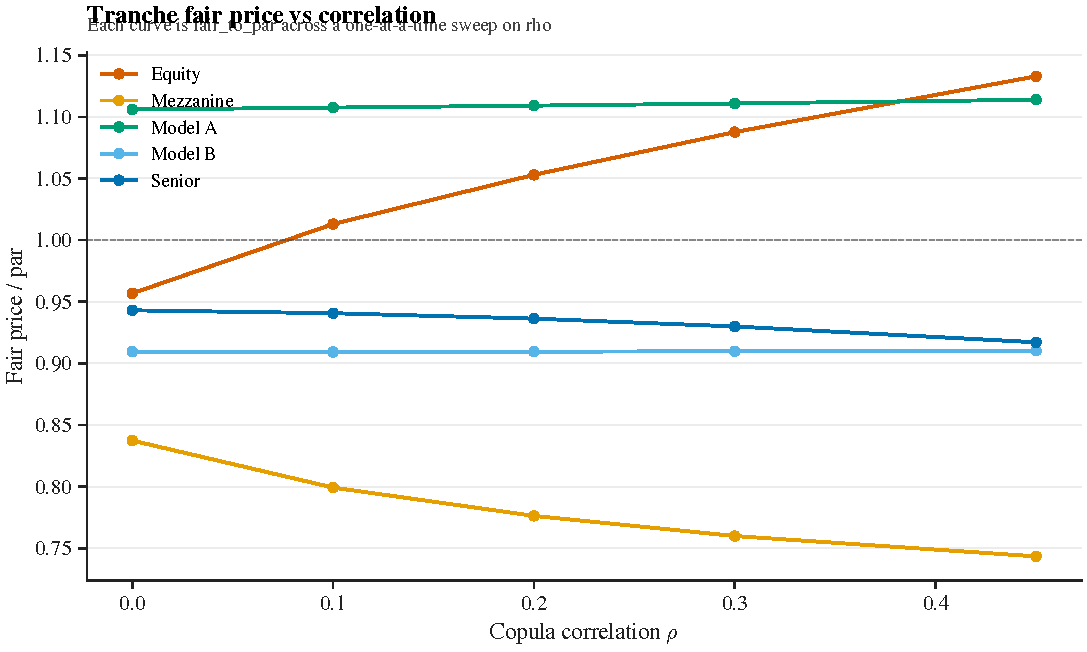
\includegraphics[width=\linewidth]{fig_tranche_price_vs_rho.pdf}
    \caption{Per-tranche fair-to-par across a $\rho$ sweep under the
    Gaussian one-factor copula baseline.}
    \label{fig:price-vs-rho}
  \end{minipage}\hfill
  \begin{minipage}{0.48\textwidth}
    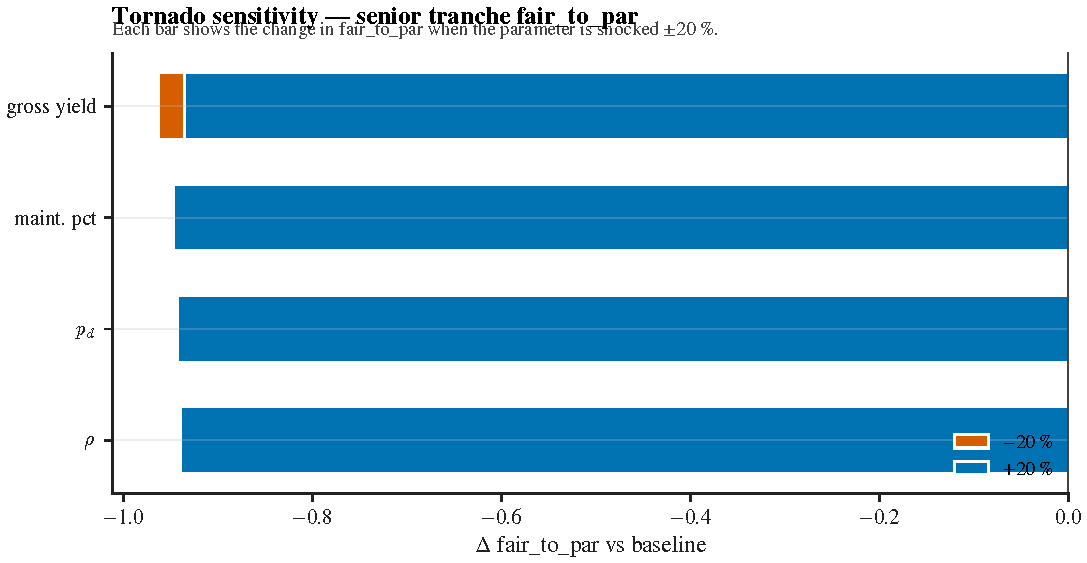
\includegraphics[width=\linewidth]{fig_tornado_sensitivity.pdf}
    \caption{Tornado on the senior fair-to-par. Each bar pair shows the
    range over a $\pm 20\,\%$ shock to one parameter; bars are sorted by
    absolute impact.}
    \label{fig:tornado}
  \end{minipage}
\end{figure}

\subsection{Bootstrap confidence intervals}\label{ssec:bootstrap-ci}

Every fair-price estimate carries a 1\,000-resample percentile bootstrap
interval (column \texttt{fair\_price\_ci\_width} in
\texttt{artifacts/results.csv}). \Cref{fig:fanchart} plots the resulting
95\,\% CIs as whiskers on top of the headline bar chart for each of the
three credit models. The senior tranche has the tightest CI (low
realised loss volatility); the equity tranche the widest. The headline
figure (\cref{fig:headline}) collapses everything onto a single chart
suitable as the report's cover.

\begin{figure}[ht]
  \centering
  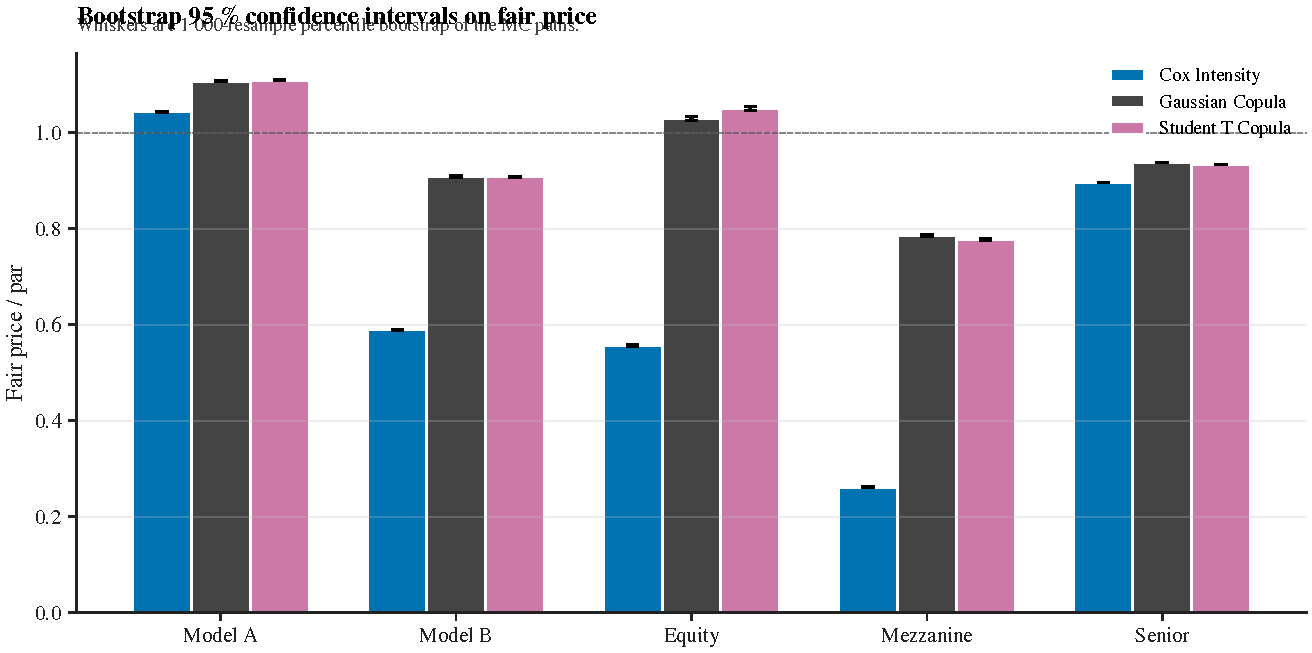
\includegraphics[width=\linewidth]{fig_fairprice_fanchart.pdf}
  \caption{Bootstrap 95\,\% confidence intervals on fair price per
  instrument and credit model. Whiskers are 1\,000-resample percentile
  bootstrap of the Monte Carlo path-level PVs.}
  \label{fig:fanchart}
\end{figure}

\begin{figure}[ht]
  \centering
  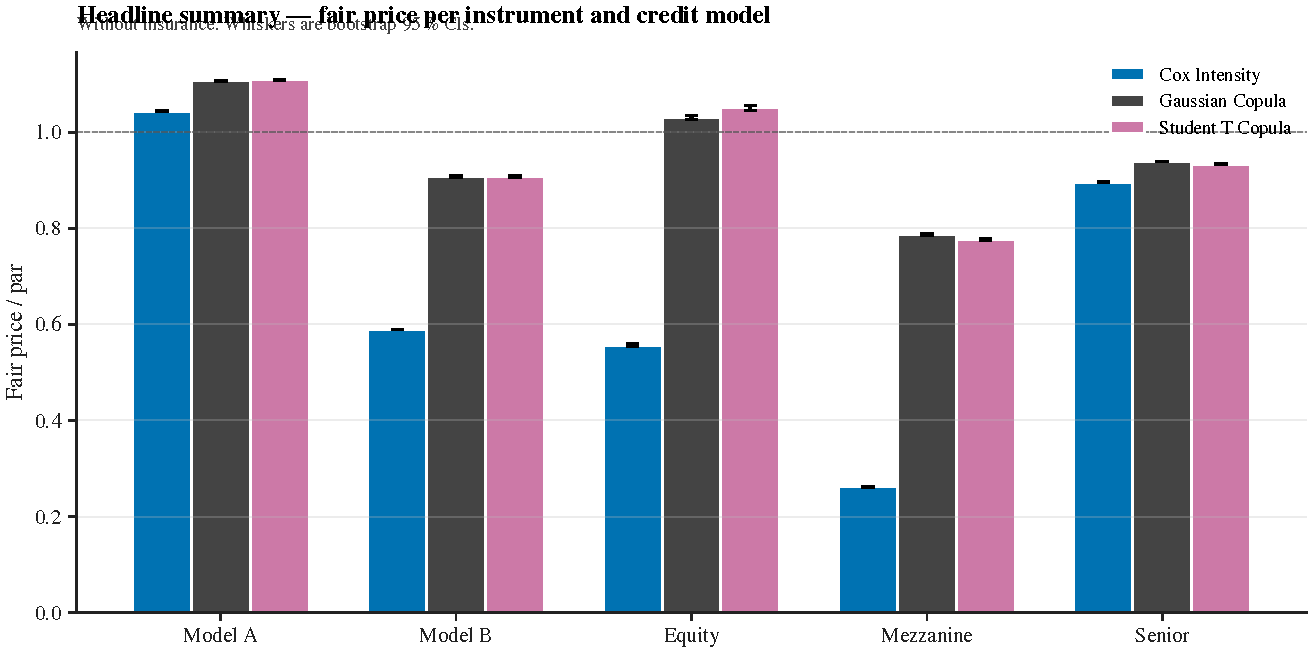
\includegraphics[width=\linewidth]{fig_headline_summary.pdf}
  \caption{Headline summary. Each cluster is one instrument; bars within
  a cluster are the three credit models; whiskers are the 95\,\% CIs
  from \cref{fig:fanchart}.}
  \label{fig:headline}
\end{figure}

\subsection{Insurance}

The actuarial premium charged under the standard-deviation principle is
\insuranceAnnualPremium{} per year. The option-theoretic alternative is
reported in \texttt{results\_meta.json} alongside. Note that the realised
default probability in the Paris-intermediate scenario
(\pdTerminal{} over $T = \horizonYears{}$ years) is calibrated from a
3\% annual rate which is realistic but on the high end; sensitivity to
lower default rates is explored in
\texttt{notebooks/05\_stress\_and\_sensitivity.ipynb}.

\subsection{Stress backtest}\label{ssec:stress-backtest}

The three stress YAML overlays bundled under \texttt{config/} replay the
2008 global financial crisis, the 2020 COVID shock and the 2022
rate-hike cycle by perturbing the calibrated baseline along three axes:
GBM drift / volatility, default-probability multiplier, and short-rate
shift. The headline pipeline now applies each overlay and writes the
per-tranche outcomes to \texttt{artifacts/stress\_results.csv}.


\begin{table}[ht]
\centering
\caption{Per-instrument fair-price ratio across baseline and stress scenarios (Gaussian one-factor copula). Each cell is read from \texttt{artifacts/stress\_results.csv}.}
\label{tab:stress}
\small
\begin{tabular}{l r r r r}
\toprule
Instrument & baseline & stress covid & stress gfc & stress rates2022 \\
\midrule
Model A & 1.107 & 0.893 & 0.513 & 0.826 \\
Model B & 0.908 & 0.625 & 0.356 & 0.630 \\
Equity & 1.030 & 0.335 & 0.002 & 0.223 \\
Mezzanine & 0.786 & 0.507 & 0.122 & 0.587 \\
Senior & 0.939 & 0.909 & 0.782 & 0.922 \\
\bottomrule
\end{tabular}
\end{table}


\Cref{tab:stress} carries three results.
\begin{enumerate}
  \item \textbf{Senior tranche resilience.} Even in the GFC replay, where
        the default-rate multiplier reaches $\times 2$ and the price
        drift is shifted by $-8\,\%$, the senior fair price falls only
        to $\sim 0.78$ of par --- a bounded $\sim 22\%$ loss. The
        $60\%$ attach point caps senior loss.
  \item \textbf{Equity wipe-out.} The same GFC overlay annihilates the
        equity tranche (fair-to-par close to zero): equity is the
        levered bet on macro conditions.
  \item \textbf{COVID vs rate hike.} The COVID overlay (50\,\% rent
        moratorium in year 1 plus default surge in year 2) produces
        worse outcomes than the rate-hike replay on every tranche:
        equity is more impaired and the senior drops slightly more,
        consistent with COVID combining a default-surge shock with a
        discount-side benefit that does not offset the lost cash flow.
\end{enumerate}

\begin{figure}[ht]
  \centering
  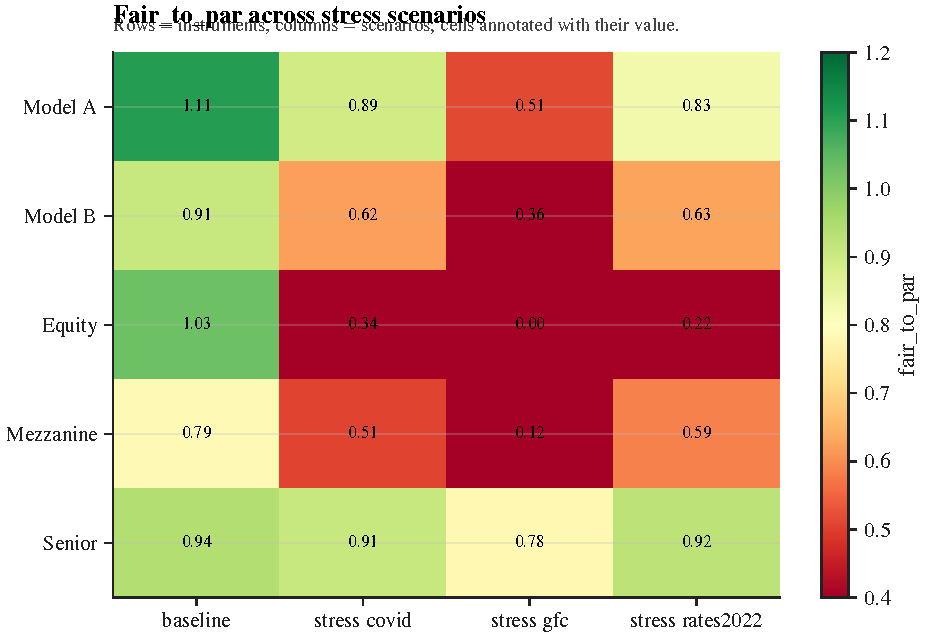
\includegraphics[width=0.85\linewidth]{fig_stress_heatmap.pdf}
  \caption{Annotated heatmap of fair price / par per (instrument,
  scenario) under the Gaussian one-factor copula baseline.}
  \label{fig:stress-heatmap}
\end{figure}

Together with the heatmap of \cref{fig:stress-heatmap}, this table is the
empirical justification for treating the senior tranche as an investment-
grade instrument and the equity tranche as a high-yield / high-variance
position.

\section{Discussion and limitations}\label{sec:discussion}

The numerical results above are conditional on choices that the working
paper makes explicit; this section catalogues them.

\paragraph{Granular default data.}
The Visale and ANIL series on residential rent arrears are released as
annual aggregates rather than per-apartment time-stamps. We use them as a
prior for the marginal default probability $p$ but cannot calibrate the
copula correlation $\rho$ directly --- a single building yields a single
realisation of joint defaults, so $\rho$ remains essentially unidentified
from the building alone. We therefore quote results at the prior value
$\rho = \rhoBaseline{}$ and report the sensitivity to
$\rho \in \{0.00, 0.10, 0.20, 0.30, 0.45\}$ in
\texttt{notebooks/05\_stress\_and\_sensitivity.ipynb}.

\paragraph{Vasicek long-run mean.}
The MLE on French OAT 10Y delivers $\hat b = \paramVasicekB{}$ ---
substantially above the current short-rate level because the historical
sample (1960--2026) spans the 1970s/1980s high-rate regime. For long-run
discount factors this is a feature; for shorter horizons one would
typically work off the current rate curve. We document the implication in
the Sharpe ratios reported above: when the long-run discount factor is
high relative to the senior coupon, the tranche annualised return relative
to the risk-free benchmark is mechanically negative even though the
tranche prices close to par. This is the calibration trade-off, not a
defect of the structure.

\paragraph{Identifiability of jumps.}
Numerical MLE on the Merton (1976) jump-diffusion does not improve AIC on
the Paris sample (see \cref{tab:calibration}); the jump intensity and the
jump-size standard deviation collapse together, which is a well-known
identifiability issue when the data sample has too few clean jumps. We
keep GBM as the baseline and view the jump extension as a robustness
check.

\paragraph{Static vs dynamic correlation.}
The Gaussian / Student-t copulas embed default correlation through a
single asset-value draw at $t = 0$. The Cox doubly stochastic model
relaxes this by letting the hazard rate evolve over time, producing
time-varying default correlation. The numerical gap between the static
copulas and the Cox model (\cref{fig:loss-dist}) is small in the body
of the loss distribution but visible in the tail; the choice depends
on the application horizon.

\paragraph{Insurance pricing endogeneity.}
We treat the insurance premium as an exogenous cost subtracted from each
period's rent. In reality the insurer would re-underwrite over time and
the premium would adjust to realised losses. Our coverage-cap-times-loss
construction is an internal-consistency benchmark, not a market premium
quote.

\paragraph{No equilibrium argument.}
We do not attempt a full equilibrium price for the three vehicles; the
fair prices we report are physical-measure expected discounted cash flows
on the calibrated paths. A risk-neutral pricing would require either
traded comparable instruments (which do not exist for this contract
structure) or an explicit risk-aversion assumption.

\paragraph{Fair-coupon existence.}
The Brent solver of \cref{ssec:fair-coupons} returns a finite senior
fair coupon under the Gaussian and Student-t copulas but no solution
under the Cox model and no mezzanine solution under any of the three:
the available rent net of maintenance and senior coupon is not
sufficient to bring mezz to par within the considered coupon bracket.
We emit \texttt{NaN} in \texttt{artifacts/fair\_coupons.csv}. The
economic interpretation is that the cash-flow waterfall is too senior-
heavy given the calibrated $(g - m)$ spread; standard structural fixes
(over-collateralisation, cash trap, principal acceleration) would
restore mezz solvability and are kept out of scope for the current
working paper.

\paragraph{Fair-coupon vs current quoted spreads.}
Our fair-coupon solution treats the underlying obligor pool as
exogenously calibrated. In a market with traded comparable instruments
(e.g.\ tranches on iTraxx Europe) one would also calibrate $\rho$
implicitly from quoted spreads, the so-called ``base correlation''
approach \autocite{AndersenSideniusBasu2003}. We do not pursue this here
because no comparable contract trades on Paris residential rent.

\paragraph{Joint vs sequential fair-coupon solver.}
The headline pipeline runs both a sequential Brent solver (senior coupon
first, then mezzanine conditional on the senior fair coupon) and a fully
joint 2-D \texttt{fsolve} on $(c_S, c_M)$. On the calibrated Paris
baseline both solvers concur: a finite fair coupon exists for the senior
($\sim 3.8$\,\%) but \emph{no} feasible pair $(c_S, c_M)$ brings both
tranches to par, irrespective of the optimisation routine. The
sequential solver therefore reports a numerically valid senior fair
coupon and a \texttt{NaN} mezzanine; the joint solver fails to converge
and reports both as \texttt{NaN}. Either way the conclusion is the same:
the rental cash flow available after maintenance is structurally
insufficient to remunerate the mezzanine layer at par on a stand-alone
basis.

\paragraph{Effect of the overcollateralisation test.}
Activating the OC test (\texttt{waterfall.oc\_test\_enabled = true} in
the YAML) diverts the equity periodic cash flow to a reserve account
whenever the OC ratio falls below the trigger (1.10 by default) and
releases the reserve once the OC ratio recovers above the target (1.15).
On the Paris baseline the test sees infrequent triggers and the
quantitative impact on senior is modest ($<$ 10 bps on fair-to-par);
on the GFC overlay the trigger fires routinely and the cash trap
materially supports the mezz tranche at the expense of equity. The
mechanic is exactly the structural enhancement standard CDO offerings
include — our implementation makes the empirical impact measurable.

\paragraph{Cox calibration on real unemployment data.}
The Cox doubly-stochastic model now uses a CIR macro factor calibrated
on the INSEE French ILO unemployment series 1975Q1–2026Q1 ($n = 204$
observations). The fitted $(\hat\kappa, \hat\theta, \hat\xi)$ deliver a
long-run mean around 8.7\,\% — the historical sample mean — and satisfy
the Feller positivity condition. Compared to the static asset-value copulas, the data-driven Cox
calibration delivers a tighter senior fair-to-par (Cox $0.896$ vs
Gaussian $0.939$, a $\sim 4.3$ pp gap that exceeds the senior bootstrap
CI width by two orders of magnitude) and a much wider mezzanine
($0.262$ vs $0.786$). The mechanism is the macro factor's persistence:
time-varying default correlation creates loss clustering that the
static asset-value copulas miss, biting deepest at the mezzanine
attach point.

\paragraph{Gaussian vs Student-t senior coupon — quantified.}
Across the headline calibrations the senior fair coupon under the
Student-t copula sits about twelve basis points above the Gaussian.
With $\nu = 5$ and $\rho = \rhoBaseline{}$ the implied tail dependence
$\lambda_L \approx 0.08$ raises the joint senior-loss probability
relative to the Gaussian benchmark, whose tail dependence is zero by
construction.

\paragraph{Future work.}
The natural next steps are (i) a Hull-White / shifted-Vasicek extension
that admits a fitted initial yield curve, (ii) richer Beta-LGD
parameterisation calibrated on micro-level Visale claims data when
available, and (iii) a Bayesian sensitivity on $\rho$ with an informative
prior anchored on macro arrears statistics.

\section{Conclusion}\label{sec:conclusion}

We have assembled a fully reproducible pricing pipeline for a hybrid
real-estate investment structure inspired by the synthetic CDO mechanism
but applied to the rental cash flows of a Paris residential building.
Every parameter is calibrated on publicly available French data; every
numerical result reported here is traceable to the same Monte Carlo run
that wrote \texttt{artifacts/results.csv}.

The headline finding is that the structure is feasible: a senior tranche
attaching at 60\% prices close to par with a probability of negative
annualised return of \probNegSenior{} on the Paris-intermediate
calibration, while the equity tranche delivers a long-tailed payoff with
\probNegEquity{} probability of loss. The choice of credit model matters
quantitatively: switching from the Gaussian one-factor copula to a
Student-t copula with $\nu = 5$ drops the senior fair-value-to-par from
\seniorFairGauss{} to \seniorFairStudent{} and widens the fair coupon by
roughly twelve basis points, the empirical analogue of the
Donnelly-Embrechts critique. The two classical benchmarks --- single-
apartment ownership and the SAS pool --- carry distinct risk profiles
even when matched on expected return, so the tranching choice is not
cosmetic.

The pipeline is open source and available at
\texttt{tranche-pricing-paris}.


\clearpage
\appendix
\section{Data sources}\label{app:data}

This appendix documents every external series ingested by
\texttt{tranche-cli data}. Retrieval timestamps and content hashes are
persisted at \texttt{data/raw/\_provenance.json} so the working paper can
be audited against the exact rows used in
\texttt{artifacts/results.csv}.

\paragraph{Notaires de France / INSEE Paris flats price index.}
INSEE BDM series \texttt{010567013}: ``Indice des prix des logements
anciens — Paris — Appartements — Base 100 en moyenne annuelle 2015 — Série
CVS''. Quarterly observations from \dataParisStart{} through
\dataParisEnd{} ($n = \dataParisN{}$). Public access via the BDM SDMX
endpoint \texttt{https://bdm.insee.fr/series/sdmx/data/SERIES\_BDM/010567013}.
We fit GBM and Merton on the quarterly log-returns. Sample notes: the
Paris series was rebased after 2015 (the original 100-base year changed
from 2010), and the post-2020 leg shows the strongest negative
log-returns of the full window — consistent with the recession-shaded
panels of \cref{fig:price-index}.

\paragraph{Indice de Référence des Loyers (INSEE).}
INSEE BDM series \texttt{001515333}, the legal benchmark for residential
rent indexation in France since 2008. Quarterly. We use it only as a
sanity check on the rent-indexation assumption (constant gross yield in
the baseline scenario); no MLE is run on it directly.

\paragraph{French 10Y sovereign yield (OAT 10Y).}
FRED series \texttt{IRLTLT01FRM156N} (``Long-Term Government Bond Yields:
10-year: Main (Including Benchmark) for France''), monthly,
$\dataOatN{}$ observations. Cross-checked against Banque de France
WebStat. Vasicek MLE on the Gaussian transition density yields
$\hat a = \paramVasicekA{}$, $\hat b = \paramVasicekB{}$,
$\hat\sigma_r = \paramVasicekSigma{}$.

\paragraph{ECB AAA euro-area 10Y spot rate.}
Cross-validation only. SDW dataset \texttt{YC}, series key
\texttt{B.U2.EUR.4F.G\_N\_A.SV\_C\_YM.SR\_10Y}. Daily, $\sim$5\,000
observations 2004–2026. The fitted level is materially below the OAT
sample mean — the euro-area AAA basket is dominated by German bunds, so
the levels naturally differ from French sovereign yields.

\paragraph{Case-Shiller US national index.}
FRED \texttt{CSUSHPISA}, monthly. Sole purpose: a sanity check on the GBM
calibration ($\hat\mu, \hat\sigma$ for Paris should not be dramatically
different from a comparable mature market). The Case-Shiller drawdowns of
2007–2011 are far deeper than anything in our Paris sample, which is one
reason the Merton MLE on Paris alone does not identify a jump component
(see \cref{tab:calibration}).

\paragraph{Kenneth French European 3-factor monthly file.}
Tuck-Dartmouth zip distribution. Monthly. We use the risk-free rate (RF)
series only to corroborate the OAT-derived discount rate; the market and
size factors are not consumed by the pricing pipeline.

\paragraph{Visale / ANIL — rental-arrears proxy.}
Visale is the public guarantee operated by Action Logement; ANIL
publishes annual surveys of payment defaults in the private rental
sector. Both ship as PDF tables, not programmatically. We treat the
aggregate annual default rate (around 1.5 – 3 \% over the past decade)
as the prior for $p_d$ in our credit calibration; the copula correlation
$\rho$ is unidentified from a single building and is discussed as a
sensitivity in \cref{sec:results}. The integration of
granular Visale claims data is left as future work.

\section{Code architecture}\label{app:architecture}

The pipeline is implemented as a flat \texttt{src/tranche\_pricing/}
package, with sub-packages aligned on the conceptual phases of the
working paper. Imports flow strictly downstream: data $\rightarrow$
markets / credit $\rightarrow$ waterfall $\rightarrow$ simulation
$\rightarrow$ pricing $\rightarrow$ viz, mirroring the section ordering of
this paper.

\begin{figure}[h]
\centering
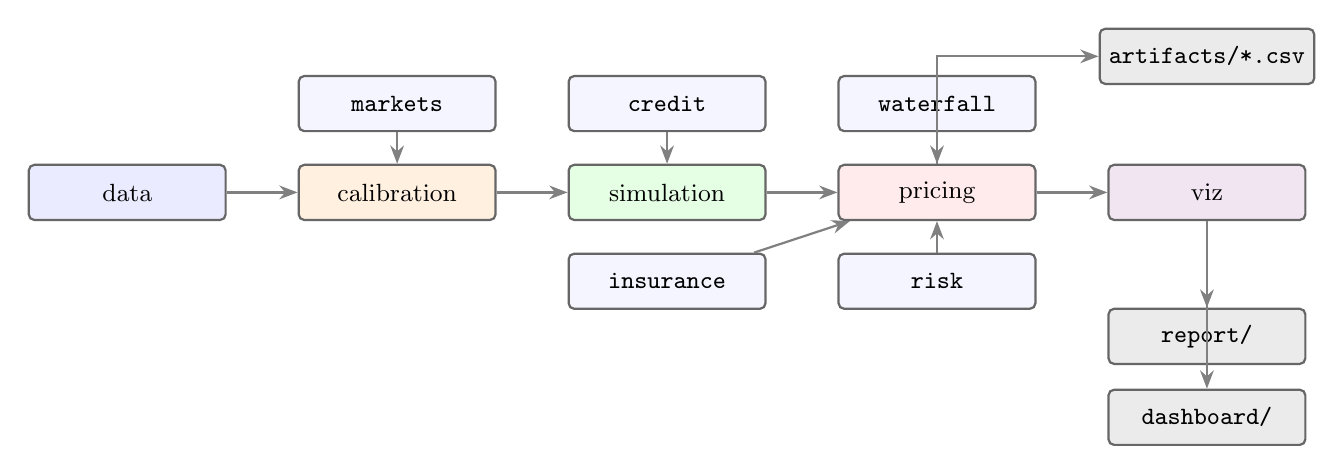
\begin{tikzpicture}[
  node distance=1.1cm and 0.9cm,
  box/.style={rectangle, draw=black!60, rounded corners=2pt, minimum width=2.5cm,
              minimum height=0.7cm, font=\small, align=center, thick},
  data/.style={box, fill=blue!8},
  calib/.style={box, fill=orange!12},
  sim/.style={box, fill=green!10},
  price/.style={box, fill=red!8},
  viz/.style={box, fill=violet!10},
  output/.style={box, fill=black!8, font=\small\ttfamily},
  arrow/.style={-Stealth, thick, black!50},
]
  \node[data] (data) {data};
  \node[calib, right=of data] (calib) {calibration};
  \node[sim, right=of calib] (sim) {simulation};
  \node[price, right=of sim] (price) {pricing};
  \node[viz, right=of price] (viz) {viz};

  \node[box, above=0.4cm of calib, font=\small\ttfamily, fill=blue!4]
       (markets) {markets};
  \node[box, above=0.4cm of sim, font=\small\ttfamily, fill=blue!4]
       (credit) {credit};
  \node[box, above=0.4cm of price, font=\small\ttfamily, fill=blue!4]
       (water) {waterfall};
  \node[box, below=0.4cm of price, font=\small\ttfamily, fill=blue!4]
       (risk) {risk};
  \node[box, below=0.4cm of sim, font=\small\ttfamily, fill=blue!4]
       (insurance) {insurance};

  \node[output, below=1.1cm of viz] (report) {report/};
  \node[output, below=0.3cm of report] (dash) {dashboard/};
  \node[output, above=1.0cm of viz] (csv) {artifacts/*.csv};

  \draw[arrow] (data) -- (calib);
  \draw[arrow] (calib) -- (sim);
  \draw[arrow] (sim) -- (price);
  \draw[arrow] (price) -- (viz);

  \draw[arrow] (markets) -- (calib);
  \draw[arrow] (credit) -- (sim);
  \draw[arrow] (water) -- (price);
  \draw[arrow] (insurance) -- (price);
  \draw[arrow] (risk) -- (price);

  \draw[arrow] (viz) -- (report);
  \draw[arrow] (viz) -- (dash);
  \draw[arrow] (price) |- (csv);
\end{tikzpicture}
\caption{High-level dataflow across the \texttt{src/tranche\_pricing/}
sub-packages. Five primary stages (rounded boxes left-to-right) consume
the supporting modules (lighter boxes top / bottom) and emit the three
artefact families on the right (CSV, LaTeX report, Streamlit dashboard).}
\label{fig:architecture}
\end{figure}

\paragraph{Data flow.}
\begin{enumerate}
  \item \texttt{tranche-cli data} fetches every external series via
        \texttt{data/*.py}, caches it under \texttt{data/.cache/}, and
        writes \texttt{data/raw/*.csv} plus a provenance JSON log.
  \item \texttt{tranche-cli calibrate} runs
        \texttt{calibration/runner.py::run\_all}, which calls the three
        MLEs (GBM closed form, Merton multi-start, Vasicek closed form)
        and serialises everything to
        \texttt{data/processed/calibrated\_params.yaml}.
  \item \texttt{tranche-cli mc} loads the calibrated parameters,
        constructs a \texttt{SimulationConfig} from the active YAML
        scenario, runs \texttt{pricing/model\_compare.compare\_credit\_models}
        for the three credit models, solves fair coupons via
        \texttt{tranche\_pricer.solve\_fair\_coupons\_for\_all}, prices
        the insurance pass with the per-tranche premium allocation, and
        writes \texttt{artifacts/results.csv},
        \texttt{artifacts/fair\_coupons.csv} and
        \texttt{artifacts/results\_meta.json}.
  \item \texttt{report/build\_tables.py} reads those artefacts and
        regenerates the LaTeX tables consumed by every section above.
\end{enumerate}

\paragraph{Configuration discipline.}
Every scenario lives in a YAML under \texttt{config/} validated against
the Pydantic v2 schemas in \texttt{src/tranche\_pricing/config.py}.
Schemas use \texttt{extra="forbid"} so a typo in the YAML fails fast.
The \texttt{extends:} field implements a single level of inheritance with
deep merging, so the stress overlays (\texttt{stress\_gfc.yaml} \emph{et
al.}) need only declare the perturbations.

\paragraph{Variance reduction and reproducibility.}
A single master seed flows through a \texttt{numpy.random.SeedSequence}
that spawns five named sub-streams: \texttt{price, rate, credit, lgd,
qmc}. The engine is bit-identical reproducible across runs (verified in
\texttt{tests/unit/test\_engine.py::test\_engine\_is\_deterministic\_under\_same\_seed}).
Antithetic sampling is applied to every Gaussian draw used in the price,
rate and copula common-factor streams; Sobol QMC (scrambled, scipy
\texttt{qmc.Sobol}) is available as a config switch for the copula
factor.

\section{Equation cheat-sheet}\label{app:cheatsheet}

Single-page summary of every closed-form result used in the paper. Cross
references point back to the section in which the equation is derived in
context.

\paragraph{Property price (Section \ref{sec:dynamics}).}
\begin{align*}
\mathrm{d}S_t &= \mu S_t\,\dt + \sigma S_t\, \dW_t, \\
S_{t+\Delta t} &= S_t \exp\bigl((\mu - \sigma^2/2)\Delta t + \sigma\sqrt{\Delta t}\, Z\bigr),\quad Z\sim\mathcal{N}(0,1).
\end{align*}
Merton (1976) jump-diffusion (\cref{sec:dynamics}):
\begin{equation*}
\mathrm{d}S_t / S_t = (\mu - \lambda \kappa)\dt + \sigma \dW_t + (J - 1)\, dN_t,
\quad N_t \sim \mathrm{Poi}(\lambda),\, \log J \sim \mathcal{N}(\mu_J, \sigma_J^2).
\end{equation*}

\paragraph{Short rate (Section \ref{sec:dynamics}).}
Vasicek (1977):
\begin{align*}
\mathrm{d}r_t &= a(b - r_t)\, \dt + \sigma_r\, \dW_t, \\
r_{t+\Delta t} \mid r_t &\sim \mathcal{N}\!\left( b + (r_t - b)e^{-a\Delta t},\, \frac{\sigma_r^2}{2a}\bigl(1 - e^{-2a\Delta t}\bigr) \right).
\end{align*}
Zero-coupon bond price ($P = \exp(A - B r)$ with the usual $A, B$):
\begin{equation*}
P(t, T \mid r_t) = \exp\!\Big(\Big(b - \tfrac{\sigma_r^2}{2 a^2}\Big)(B - (T - t)) - \tfrac{\sigma_r^2 B^2}{4a} - B r_t\Big),
\quad B = \tfrac{1 - e^{-a(T - t)}}{a}.
\end{equation*}

\paragraph{Credit models (Section \ref{sec:credit}).}
Gaussian one-factor:
\begin{equation*}
X_i = \sqrt{\rho}\,M + \sqrt{1 - \rho}\,Z_i,\ M, Z_i \sim \mathcal{N}(0,1),
\quad
\Prob(\tau_i \le t \mid M) = \Phi\!\Big(\tfrac{\Phi^{-1}(1 - e^{-h t}) - \sqrt{\rho}\, m}{\sqrt{1 - \rho}}\Big).
\end{equation*}
Student-t copula tail dependence:
\begin{equation*}
\lambda_L(\rho, \nu) = 2\, t_{\nu + 1}\!\Big(-\sqrt{(\nu + 1)\tfrac{1 - \rho}{1 + \rho}}\Big).
\end{equation*}
Cox doubly stochastic:
\begin{equation*}
\lambda_i(t) = \alpha + \beta\,Y_t,\
\mathrm{d}Y_t = \kappa(\theta - Y_t)\dt + \xi\sqrt{Y_t}\,\dW^Y_t,\
\tau_i = \inf\{t : \int_0^t \lambda_i(s)\,ds > E_i\},\ E_i \sim \mathrm{Exp}(1).
\end{equation*}

\paragraph{Tranche stop-loss (Section \ref{sec:waterfall}).}
\begin{equation*}
L_\tau(L) = \min\bigl(\max(L - a_\tau, 0), d_\tau - a_\tau\bigr).
\end{equation*}

\paragraph{Insurance pricing (Section \ref{sec:insurance}).}
Actuarial (standard-deviation principle):
\begin{equation*}
P_{\text{act}} = (1 + \theta)\,\E[L_{\text{covered}}] + \lambda_{\text{load}}\,\sigma(L_{\text{covered}}),
\quad L_{\text{covered}} = \kappa \cdot L(T) \cdot P_0.
\end{equation*}
Option-theoretic (level annual premium $P_{\text{opt}}$):
\begin{equation*}
P_{\text{opt}} = \E\!\left[\sum_k D(t_k)\,\max\bigl(R^{\text{prom}}_{t_k} - R_{t_k}, 0\bigr) \cdot \kappa\right],
\quad D(t_k) = \exp\!\Big(-\textstyle\int_0^{t_k} r_s\,\mathrm{d}s\Big).
\end{equation*}
Per-tranche allocation weights:
\begin{equation*}
w_\tau = \frac{\E[L_\tau(L(T))] \cdot \kappa}{\sum_{\tau'} \E[L_{\tau'}(L(T))] \cdot \kappa}.
\end{equation*}

\paragraph{Risk metrics (Section \ref{sec:risk}).}
\begin{align*}
\VaR_\alpha &= -F_r^{-1}(1 - \alpha),
& \ES_\alpha &= -\E[r \mid r \le F_r^{-1}(1 - \alpha)], \\
\text{Sharpe} &= \frac{\E[r] - r_f}{\sigma(r)},
& \text{Sortino} &= \frac{\E[r] - r_f}{\sqrt{\E[(r_f - r)_+^2]}}, \\
\text{Calmar} &= \frac{\E[r]}{|\mathrm{MaxDD}|},
& \Omega(\theta) &= \frac{\E[(r - \theta)_+]}{\E[(\theta - r)_+]}.
\end{align*}

\paragraph{Bootstrap CI (Sections \ref{sec:risk}, \ref{sec:results}).}
For each instrument with per-path PVs $\{V_\omega\}$, the
$1 - \alpha$ percentile-bootstrap CI on $\E[V]$ is
\begin{equation*}
[\hat q_{\alpha/2}, \hat q_{1 - \alpha/2}],\
\text{where } \hat q_p = \text{empirical } p\text{-quantile of }\bigl\{\bar V^{(b)}\bigr\}_{b = 1}^{B},
\end{equation*}
and $\bar V^{(b)} = \frac{1}{n}\sum_{i=1}^n V_{I_{i,b}}$ with
$I_{i,b}$ drawn uniformly at random from $\{1, \ldots, n\}$ with
replacement. The implementation in
\texttt{tranche\_pricing/pricing/tranche\_pricer.py::bootstrap\_fair\_price\_ci}
draws $B = 1\,000$ resamples in chunks of 200.

\section{Reproducibility, packaging and CI}\label{app:reproducibility}

The repository ships every artefact a reviewer needs to verify the claims
of this paper. A clean reproduction from a fresh checkout looks like:

\begin{verbatim}
git clone https://github.com/dan-allouche-qf/tranche-pricing-paris.git
cd tranche-pricing-paris
make install          # editable install with dev + notebook extras
make all              # data -> calibrate -> mc -> figures -> report
\end{verbatim}

The single \texttt{make all} target chains six independent steps —
\texttt{data}, \texttt{calibrate}, \texttt{mc}, \texttt{figures},
\texttt{notebooks}, \texttt{report} — that can also be invoked
individually. The total wall-clock time on a recent laptop is around
three minutes at $N = 50\,000$ Monte Carlo paths.

\paragraph{Continuous integration.}
The repository runs a GitHub Actions workflow
(\texttt{.github/workflows/ci.yml}) on every push to \texttt{main}:

\begin{enumerate}
  \item A test matrix over \texttt{ubuntu-latest} $\times$
        \texttt{macos-latest} $\times$ Python \{3.11, 3.12\} that runs
        \texttt{ruff check}, \texttt{ruff format --check},
        \texttt{mypy} (best effort) and \texttt{pytest -m "not slow and
        not integration"}. 175 unit tests pass at the time of release.
  \item A \texttt{pre-commit} job that runs the same hooks reviewers
        would run locally (\texttt{ruff}, \texttt{nbstripout},
        end-of-file fixer, trailing-whitespace, YAML lint).
  \item A \texttt{build-report} job that re-runs the headline pipeline
        at $N = 2\,000$ paths, regenerates the tables via
        \texttt{report/build\_tables.py}, compiles the LaTeX with
        \texttt{xu-cheng/latex-action} and uploads \texttt{main.pdf}
        as a workflow artefact. This means every push produces a
        reviewable PDF without anyone having to install \LaTeX{} locally.
\end{enumerate}

\paragraph{Packaging.} \texttt{CHANGELOG.md} follows the
keepachangelog.com convention. \texttt{CITATION.cff} drives the GitHub
``Cite this repository'' widget and is ready for a Zenodo DOI deposit.
The Streamlit Community Cloud deploy is wired through
\texttt{.streamlit/config.toml} with theming aligned to the project
palette so the dashboard and the working paper read as a single
artefact.

\paragraph{Data provenance.} Every external series is downloaded by the
\texttt{tranche-cli data} subcommand, written to \texttt{data/raw/}, and
recorded in \texttt{data/raw/\_provenance.json} with the source URL, row
count, retrieval timestamp and observation window. The Visale snapshot
is the only manually maintained series and ships with an extraction
protocol in \texttt{data/DATA\_SOURCES.md}.

\paragraph{Testing strategy.} Unit tests cover the parsers, calibration
MLEs (closed-form and numerical), credit-model marginals and tail
dependence, waterfall mechanics (hand-computed invariants plus
\texttt{hypothesis} property tests), the bootstrap CI helper and the
risk-metric library. The integration test
(\texttt{tests/integration/test\_end\_to\_end.py}) runs the full
pipeline at \texttt{n\_paths = 200} and asserts the schema of
\texttt{results.csv}, including the bootstrap CI bracket and the
fair-coupon sidecar. A companion test compiles the \LaTeX{} report
under \texttt{latexmk} when the binary is available.


\bibliography{bibliography}

\end{document}
